\chapter{Appendix to Chapter 3}
\label{chap:appendix_ch3}

\section{Computing the matrix exponential}
\label{sec:mtx_exp}
The transition probability matrix (TPM), $ \bP(t) $, for a time--homogeneous CTMC over an interval of length $ t $, solves the matrix differential equation \[ \frac{\rmd}{\rmd t}\bP(t) = \bLambda\bP(t),\hspace{0.2in} \mathrm{s.t.\ }\mathbf{P}(0) = \mathbf{I}, \] where $ \bLambda $ is the transition rate matrix for the CTMC and $ \mathbf{I} $ is an identity matrix of the same size as $ \bLambda $ \citep{wilkinson2011stochastic}.  Therefore, $ \bP $ is computed using the matrix exponential solution of the above differential equation, $ \bP = \exp(t\bLambda) $. This is the most intensive step in our algorithm. However, we may lessen the computational burden to a large extent by leveraging the fact that we are computing the matrix exponential for the same rate matrix for possibly many values of $ t $. Therefore, computing the matrix exponential using the eigen decomposition of $ \bLambda $ and caching the resulting eigenvalues and eigenvectors will be relatively efficient \citep{moler2003nineteen}. We outline this computation in the following two cases: when the eigenvalues of $ \bLambda $ are all real (e.g. as with the SIR and SEIR models), and when $ \bLambda $ has complex eigenvalues (e.g. as is possibly the case with the SIRS model).

\subsection{Case 1: $ \bLambda $ has real eigenvalues}
Suppose that $ \bLambda_{n\times n} =  \mathbf{UVU}^{-1}$, where $ \mathbf{V} $ is a diagonal matrix of eigenvalues, $ v_1,\dots,v_n $, and $ \mathbf{U} $ is the matrix whose columns are the corresponding right eigenvectors. Then, \[ \e^{t\mathbf{V}} = \diag(\e^{v_1t},\dots,\e^{v_nt}). \] That $ \mathbf{U} $ is nonsingular yields \[ \e^{t\bLambda} = \mathbf{U} \e^{t\mathbf{V}}\mathbf{U}^{-1}. \] 

\subsection{Case 2: $ \bLambda $ has complex eigenvalues}
In the event that $ \bLambda $ has complex eigenvalues, we may obtain a real-valued TPM by transforming $ \bLambda $ into its real canonical form \citep{hirsch2013differential}. Suppose that $ \bLambda $ has $ r $ real eigenvalues, $ v_1,\dots,v_r $, with corresponding real eigenvectors, $ \bu_1,\dots,\bu_r $, and $ n-r $ pairs of complex conjugate eigenvalues. Let $ (\bu_j|\bw_j) $ denote the real and imaginary parts of the eigenvector corresponding to the $ j^{th} $ eigenvalue, $ \alpha_j + i\beta_j $, for $ j = r+1,\dots,n $, and define the matrix $ \mathbf{T} = \left (\bu_1|\dots|\bu_r|\bu_{r+1}|\bw_{r+1}|\dots|\bu_n|\bw_n\right ) $. 
The real canonical form for a rate matrix with complex eigenvalues can now be written as $ \mathbf{V} = \mathbf{T}^{-1}\bLambda \mathbf{T} $, where $ \mathbf{V} = \diag(v_1,\dots,v_r,\mathbf{B}_{r+1},\dots, \mathbf{B}_n) $, and each $ \mathbf{B}_j,\ j=r+1,\dots,n $ is given by 
\[ \mathbf{B}_j = \left (\begin{array}{cc}
\alpha_j & \beta_j \\
-\beta_j & \alpha_j
\end{array}\right ), \]
which implies that 
\[ \e^{t\mathbf{B}_j} = \e^{\alpha_jt}\left (\begin{array}{cc}
\cos(\beta_jt) & \sin(\beta_jt) \\
-\sin(\beta_jt) & \cos(\alpha_j)
\end{array}\right ), \]
and hence $ \e^{t\mathbf{V}} = \diag(\e^{v_1t},\dots,\e^{v_rt},\e^{t\mathbf{B}_{r+1}},\dots, \e^{t\mathbf{B}_n}) $. Therefore, we can compute the matrix exponential of $ t\bLambda $ as $ \e^{t\bLambda} = \mathbf{T}\e^{t\mathbf{V}}\mathbf{T}^{-1}. $

\newpage
\section{Conjugate priors for SIR, SEIR, and SIRS model parameters}
\label{sec:bda_priors}

\begin{table}[htbp]
	\begin{center}
		\small
		\begin{tabular}{clcc}
			\hline \rule[-2ex]{0pt}{5.5ex} Parameter & \shortstack{\\Conjugate \\ Prior Dist.} & \shortstack{\\Prior\\ Hyperparameters} & Full Conditional Hyperparameters \\ 
			
			\hline \hline
			
			\rule[-2ex]{0pt}{5.5ex} $R_0$ & Beta$ ^\prime $ & $ a_\beta,\ a_\mu,\ 1,\ \frac{b_\mu N}{b_\beta} $& ---\\
			
			\hline \rule[-2ex]{0pt}{5.5ex} $\beta$ & Gamma & $a_\beta,\  b_\beta$ & $a_\beta + \sum_{j=1}^{M}\ind{\tau_j\corresponds I},\  b_\beta + \sum_{j=1}^{M}S_{\tau_{j-1}}I_{\tau_{j-1}}(\tau_j - \tau_{j-1})$\\ 
			
			\hline \rule[-2ex]{0pt}{5.5ex} $\mu$ & Gamma & $a_\mu,\ b_\mu$ & $a_\mu + \sum_{j=1}^{M}\ind{\tau_j \corresponds R},\  b_\mu + \sum_{j=1}^{M}I_{\tau_{j-1}}(\tau_j - \tau_{j-1})$\\ 
			
			\hline \rule[-2ex]{0pt}{5.5ex} $\rho$ & Beta & $a_\rho,\ b_\rho$ & $a_\rho + \sum_{j=1}^{L}Y_{t_j},\ b_\rho + \sum_{j=1}^{L}(I_{t_j} - Y_{t_j})$\\ 
			
			\hline \rule[-2ex]{0pt}{5.5ex} $\mathbf{p}_{t_1}$ & Dirichlet & $a_{S},\ b_{I},\ c_{R}$ & $a_{S} + S_{t_1},\ b_{I} + I_{t_1},\ c_{R} + R_{t_1}$\\ 
			\hline 
		\end{tabular}
		\caption[Conjugate priors and full conditionals for SIR model parameters.]{Prior and full conditional distributions for SIR model parameters. $ \beta $ is the per--contact infectivity rate, $ \mu $ is the recovery rate, $ \rho $ is the binomial sampling probability, and $ \bp_{t_1} $ is the vector of initial state probabilities. Gamma priors are parameterized with rates, so a Gamma($ a,b $) distribution has mean $ a/b $. The Beta prime prior for $ R_0 = \beta N / \mu $ is the implied prior induced by the prior distributions for $ \beta $ and $ \mu $. The indicators $ \ind{\tau_j \corresponds I} $ and $\ind{\tau_j \corresponds R} $ equal 1 if $ \tau_j $ corresponds to a time when an individual becomes infected or recovers.}
		\label{tab:SIR_priors}
	\end{center}
\end{table}


\begin{table}[htbp]
	\begin{center}
		\small
		\begin{tabular}{clcc}
			\hline \rule[-2ex]{0pt}{5.5ex} Parameter & \shortstack{\\Conjugate \\ Prior Dist.} & \shortstack{\\Prior\\ Hyperparameters} & Full Conditional Hyperparameters \\ 
			
			\hline \hline
			
			\rule[-2ex]{0pt}{5.5ex} $R_0$ & Beta$ ^\prime $ & $ a_\beta,\ a_\mu,\ 1,\ \frac{b_\mu N}{b_\beta} $& ---\\
			
			\hline \rule[-2ex]{0pt}{5.5ex} $\beta$ & Gamma & $a_\beta,\  b_\beta$ & $a_\beta + \sum_{j=1}^{M}\ind{\tau_j \corresponds E},\  b_\beta + \sum_{j=1}^{M}S_{\tau_{j-1}}I_{\tau_{j-1}}(\tau_j - \tau_{j-1})$\\
			
			\hline \rule[-2ex]{0pt}{5.5ex} $\gamma$ & Gamma & $a_\gamma,\ b_\gamma$ & $a_\gamma + \sum_{j=1}^{M}\ind{\tau_j\corresponds I},\  b_\gamma + \sum_{j=1}^{M}E_{\tau_{j-1}}(\tau_j - \tau_{j-1})$\\ 
			
			\hline \rule[-2ex]{0pt}{5.5ex} $\mu$ & Gamma & $a_\mu,\ b_\mu$ & $a_\mu + \sum_{j=1}^{M}\ind{\tau_j \corresponds R},\  b_\mu + \sum_{j=1}^{M}I_{\tau_{j-1}}(\tau_j - \tau_{j-1})$\\ 
			
			\hline \rule[-2ex]{0pt}{5.5ex} $\rho$ & Beta & $a_\rho,\ b_\rho$ & $a_\rho + \sum_{j=1}^{L}Y_{t_j},\ b_\rho + \sum_{j=1}^{L}(I_{t_j} - Y_{t_j})$\\ 
			
			\hline \rule[-2ex]{0pt}{5.5ex} $\mathbf{p}_{t_1}$ & Dirichlet & $a_{S},\ b_{I},\ c_{R}$ & $a_{S} + S_{t_1},\ b_{I} + I_{t_1},\ c_{R} + R_{t_1}$\\ 
			\hline 
		\end{tabular}
		\caption[Conjugate priors and full conditionals for SEIR model parameters.]{Prior and full conditional distributions for SEIR model parameters. $ \beta $ is the per--contact infectivity rate, $ \gamma $ is the rate at which an exposed individual becomes infectious, $ \mu $ is the recovery rate, $ \rho $ is the binomial sampling probability, and $ \bp_{t_1} $ is the vector of initial state probabilities. Gamma priors are parameterized with rates, so a Gamma($ a,b $) distribution has mean $ a/b $. The Beta prime prior for $ R_0 = \beta N / \mu $ is the implied prior induced by the prior distributions for $ \beta $ and $ \mu $. The indicators $ \ind{\tau_j \corresponds E} $, $ \ind{\tau_j \corresponds I} $ and $\ind{\tau_j \corresponds R} $ equal 1 if $ \tau_j $ corresponds to a time when an individual becomes exposed, becomes infectious, or recovers.}
		\label{tab:SEIR_priors}
	\end{center}
\end{table}


\begin{table}[htbp]
	\begin{center}
		\small
		\begin{tabular}{clcc}
			\hline \rule[-2ex]{0pt}{5.5ex} Parameter & \shortstack{\\Conjugate \\ Prior Dist.} & \shortstack{\\Prior\\ Hyperparameters} & Full Conditional Hyperparameters \\ 
			
			\hline \hline
			
			\rule[-2ex]{0pt}{5.5ex} $R_0$ & Beta$ ^\prime $ & $ a_\beta,\ a_\mu,\ 1,\ \frac{b_\mu N}{b_\beta} $& ---\\
			
			\hline \rule[-2ex]{0pt}{5.5ex} $\beta$ & Gamma & $a_\beta,\  b_\beta$ & $a_\beta + \sum_{j=1}^{M}\ind{\tau_j \corresponds E},\  b_\beta + \sum_{j=1}^{M}S_{\tau_{j-1}}I_{\tau_{j-1}}(\tau_j - \tau_{j-1})$\\
			
			\hline \rule[-2ex]{0pt}{5.5ex} $\mu$ & Gamma & $a_\mu,\ b_\mu$ & $a_\mu + \sum_{j=1}^{M}\ind{\tau_j \corresponds R},\  b_\mu + \sum_{j=1}^{M}I_{\tau_{j-1}}(\tau_j - \tau_{j-1})$\\ 
			
			\hline \rule[-2ex]{0pt}{5.5ex} $\gamma$ & Gamma & $a_\gamma,\ b_\gamma$ & $a_\gamma + \sum_{j=1}^{M}\ind{\tau_j\corresponds L},\  b_\gamma + \sum_{j=1}^{M}R_{\tau_{j-1}}(\tau_j - \tau_{j-1})$\\ 
			
			\hline \rule[-2ex]{0pt}{5.5ex} $\rho$ & Beta & $a_\rho,\ b_\rho$ & $a_\rho + \sum_{j=1}^{L}Y_{t_j},\ b_\rho + \sum_{j=1}^{L}(I_{t_j} - Y_{t_j})$\\ 
			
			\hline \rule[-2ex]{0pt}{5.5ex} $\mathbf{p}_{t_1}$ & Dirichlet & $a_{S},\ b_{I},\ c_{R}$ & $a_{S} + S_{t_1},\ b_{I} + I_{t_1},\ c_{R} + R_{t_1}$\\ 
			\hline 
		\end{tabular}
		\caption[Conjugate priors and full conditionals for SIRS model parameters.]{Prior and full conditional distributions for SIRS model parameters. $ \beta $ is the per--contact infectivity rate, $ \mu $ is the recovery rate, $ \gamma $ is the rate at which a recovered individual loses immunity, $ \rho $ is the binomial sampling probability, and $ \bp_{t_1} $ is the vector of initial state probabilities. Gamma priors are parameterized with rates, so a Gamma($ a,b $) distribution has mean $ a/b $. The Beta prime prior for $ R_0 = \beta N / \mu $ is the implied prior induced by the prior distributions for $ \beta $ and $ \mu $. The indicators $ \ind{\tau_j \corresponds I} $, $\ind{\tau_j \corresponds R} $, and $ \ind{\tau_j \corresponds L} $  equal 1 if $ \tau_j $ corresponds to a time when an individual becomes infected, recovers, or loses immunity.}
		\label{tab:SIRS_priors}
	\end{center}
\end{table}

\section{Simulation 1 --- Inference Under Various Epidemic\\ Dynamics --- Setup and Additional Results}
\label{sec:bda_sim1_details}
\subsection{Simulation details for the SIR model}
We simulated an epidemic in a population of 750 individuals, 90\% of whom were initially susceptible and 3\% of whom were initially infected. Prevalence was observed with detection probability $ \rho=0.2 $ at weekly intervals over a four month period which captured both the exponential growth and decline of the epidemic. The mean infectious period was $ 1/\mu = 7 $ days and the per-contact infectivity rate was 0.00035, which combined to give a basic reproductive number was $ R_0 = \beta N /\mu \approx 1.8$.

We ran three chains for 100,000 iterations each, sampling the paths for 75 subjects, chosen uniformly at random, per MCMC iteration. We discarded the first 10 iterations from each chain as burn-in. Priors for the rate parameters (summarized in Table \ref{tab:sim1_sir_priors}) were scaled so that the prior mass spanned a reasonable range of values, but were otherwise mild. Similarly, the prior for the binomial sampling probability reflected a general prior belief that fewer than 40\% of cases were detected. The prior for the initial distribution parameters was informative, and was chosen as such because of the paucity of data available for estimation of the initial distribution parameters.

\begin{table}[htbp]
	\centering
	\begin{tabular}{lll}
		\hline
		Param. & True Value & Prior distribution \\ 
		\hline
		$ R_0 $ & 1.8 & Beta$ ^\prime $(0.3, 1, 1, 6) \\
		$ \beta $ & 0.00035 & Gamma$ (0.3, 1000) $ \\ 
		$ \mu $ & 0.14 & Gamma(1, 8)  \\ 
		$ \bp_{t_1} $ & (0.9, 0.03, 0.07) & Dirichlet(90, 2, 5)  \\ 
		$ \rho $ & 0.2 & Beta(2, 7) \\
		\hline
	\end{tabular}
	\caption[Simulation 1 priors for SIR model parameters.]{Prior distributions for SIR model and measurement process parameters. The prior for $ R_0 $ is the induced prior implied by $ \beta $ and $ \mu $. The per--contact infectivity rate is $ \beta $, the recovery rate is $ \mu $, the binomial sampling probability is $ \rho $, and the initial state probabilities are $ \bp_{t_1} $.}
	\label{tab:sim1_sir_priors}
\end{table}

We also fit the SIR model to the data using PMMH. We ran two sets of three MCMC chains with the PMMH algorithm for 50,000 iterations each with 100 particles per chain, and discarded the first 100 iterations as burn-in. The first set of chains simulated particle paths approximately using $ \tau $--leaping with a time step of two hours, while the second chain simulated paths exactly via Gillespie's direct algorithm. Parameters were updated using random walk Metropolis--Hastings (RWMH) with a proposal covariance matrix estimated from an initial run of 5,000 iterations using an adaptive RWMH algorithm with a target acceptance rate of 23.4\%. We updated parameters on transformed scales in  order to remove restrictions on the parameter space, applying a log transformation to $ \beta $ and $ \mu $, a logit transformation to $ \rho $, and a generalized logit transformation to $ \bp_{t_1} $.

\newpage
\subsection{Additional results and MCMC diagnostics for the SIR model}
\begin{table}[htbp]
	\centering
	\begin{tabular}{lrrrr}
		\hline
		Method & Chain & Hours & ESS & ESS per CPU time \\ 
		\hline
		BDA &  1 & 9.9 & 87.7 & 8.8 \\ 
		BDA &  2 & 8.7 & 67.9 & 7.8 \\ 
		BDA &  3 & 8.5 & 63.8 & 7.5 \\ 
		PMMH--A &  1 & 0.6 & 1847.4 & 2871.6 \\ 
		PMMH--A &  2 & 0.6 & 1942.2 & 2995.7 \\ 
		PMMH--A &  3 & 0.7 & 1876.6 & 2615.9 \\ 
		PMMH--E &  1 & 26.1 & 1568.3 & 60.1 \\ 
		PMMH--E &  2 & 20.4 & 2123.7 & 104.0 \\ 
		PMMH--E &  3 & 20.5 & 1849.4 & 90.2 \\ 
		\hline
	\end{tabular}
	\caption[Simulation 1 log--posterior effective sample sizes and run times.]{Run times, log--posterior effective sample sizes (ESSs), and effective sample sizes per CPU time measure in hours (ESS.per.CPU.time). BDA indicates our Bayesian data augmentation algorithm, PMMH--A indicates PMMH with paths simulated approximately via $ \tau $--leaping algorithm, and PMMH--E indicates PMMH with paths simulated exactly using Gillespie's direct algorithm. The BDA chains were run for 100,000 iterations each, while the PMMH chains were run for 50,000 iterations following a tuning run of 5,000 iterations.}
	\label{tab:sim1_sir_ess}
\end{table}

\begin{figure}[htbp]
	\centering
	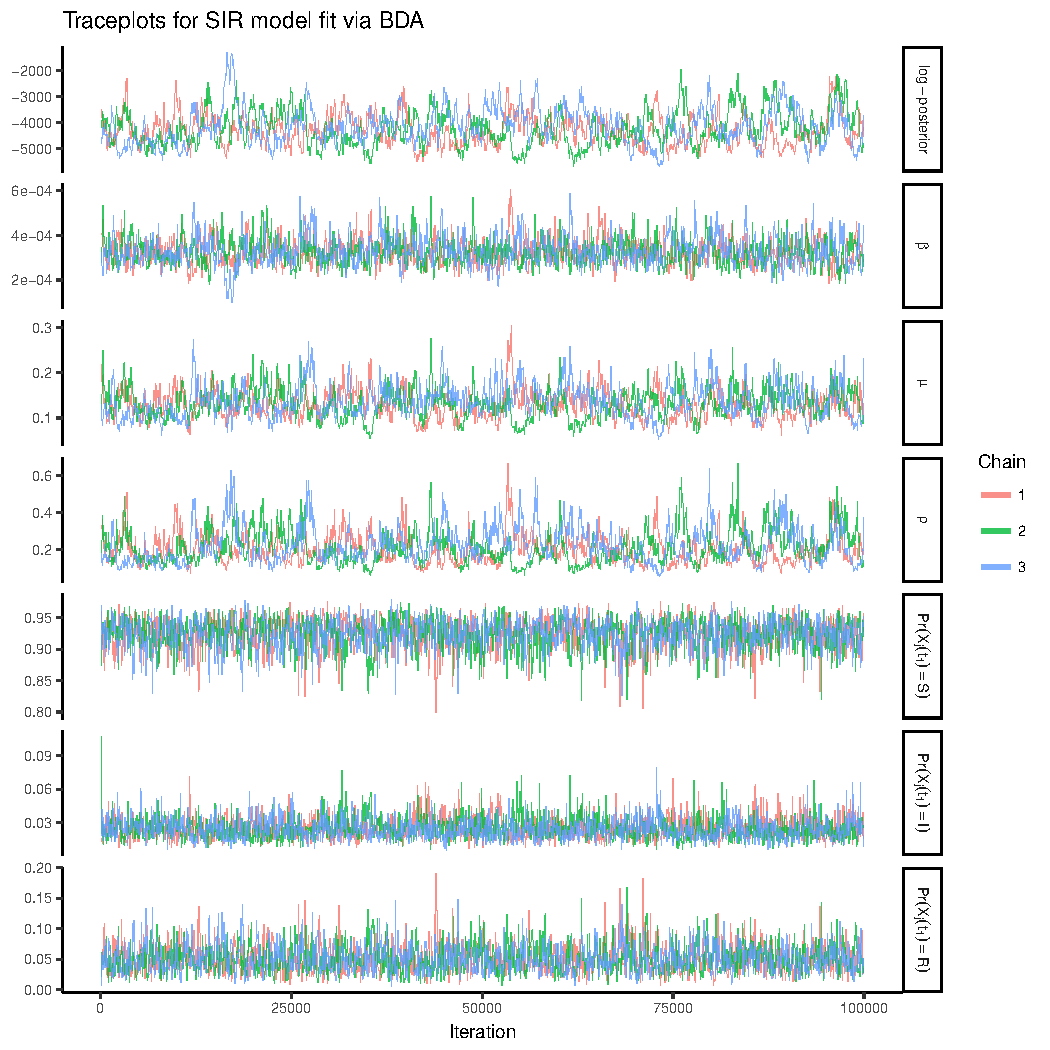
\includegraphics[width=0.9\linewidth]{figures/sir_bda_traceplots}
	\caption[Simulation 1 MCMC traceplots for an SIR model fit using Bayesian data augmentation.]{Traceplots of the log--posterior and model parameters for the SIR model fit using Bayesian data augmentation following an initial burn--in of 10 iterations. $ \beta $ denotes the per--contact infectivity rate, $ \mu $ is the recovery rate, $ \rho $ is the binomial sampling probability. Traceplots are thinned to display every 50\textsuperscript{th} iteration.}
	\label{fig:sirbdatraceplots}
\end{figure}

\begin{figure}[htbp]
	\centering
	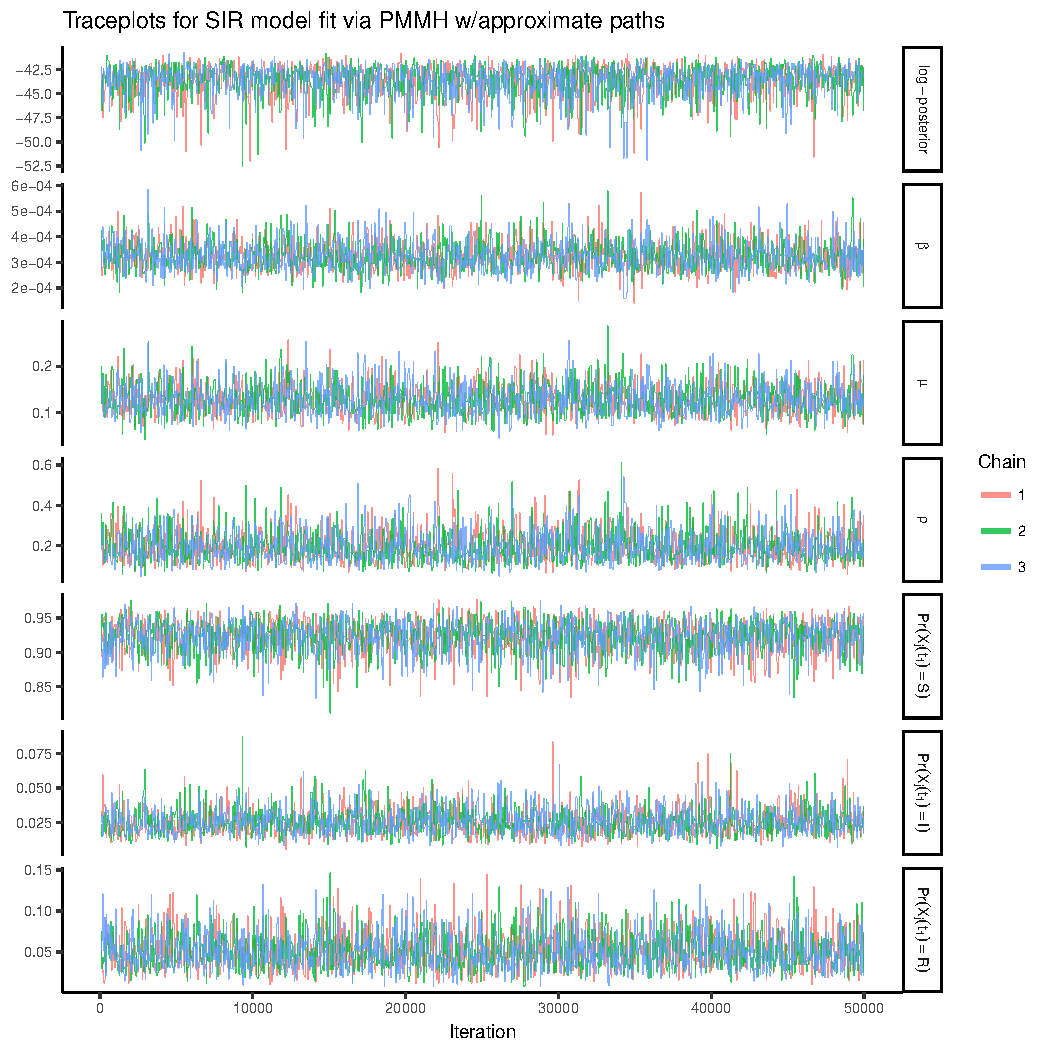
\includegraphics[width=0.9\linewidth]{figures/sir_pomp_approx_traceplots}
	\caption[Simulation 1 MCMC traceplots for an SIR model fit using PMMH with approximate particle paths.]{Traceplots of the log--posterior and model parameters for the SIR model fit using PMMH with 100 particles and a time step of 8 hours, following a tuning run of 5,000 iterations used to estimate the covariance matrix for the RWMH and an initial burn--in of 100 iterations. $ \beta $ denotes the per--contact infectivity rate, $ \mu $ is the recovery rate, $ \rho $ is the binomial sampling probability. Traceplots are thinned to display every 50\textsuperscript{th} iteration.}
	\label{fig:sirpompapproxtraceplots}
\end{figure}

\begin{figure}[htbp]
	\centering
	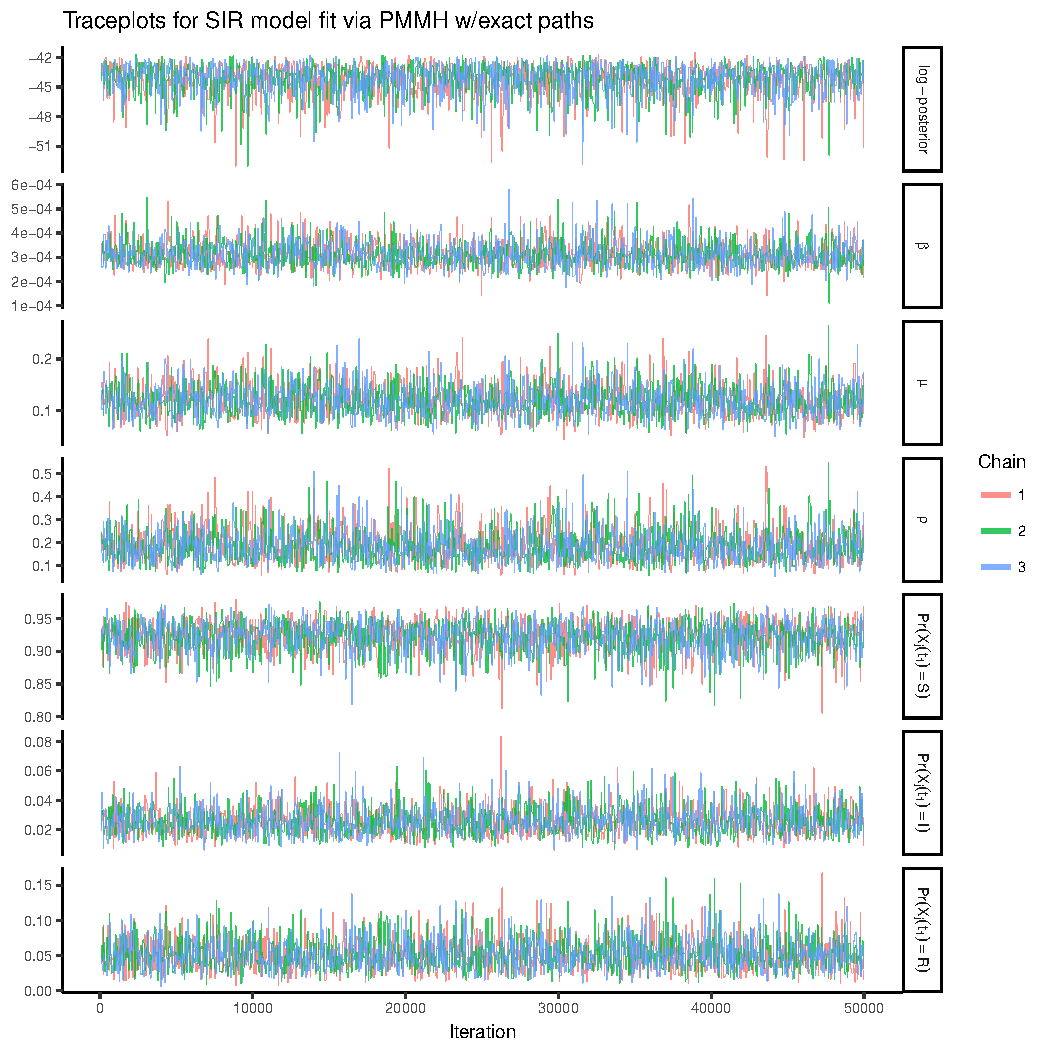
\includegraphics[width=0.9\linewidth]{figures/sir_pomp_exact_traceplots}
	\caption[Simulation 1 MCMC traceplots for an SIR model fit using PMMH with exact particle paths.]{Traceplots of the log--posterior and model parameters for the SIR model fit using PMMH with 100 particles, following a tuning run of 5,000 iterations used to estimate the covariance matrix for the RWMH and an initial burn--in of 100 iterations. $ \beta $ denotes the per--contact infectivity rate, $ \mu $ is the recovery rate, $ \rho $ is the binomial sampling probability. Traceplots are thinned to display every 50\textsuperscript{th} iteration.}
	\label{fig:sirpompexacttraceplots}
\end{figure}

\newpage
\subsection{Simulation details for the SEIR model}
\label{subsec:bda_seir_sim1_details}
We simulated an outbreak under near-endemic SEIR dynamics, with $ R_0 = \beta N / \mu = 1.05 $, in a population of 500 individuals. The outbreak was initiated by a single infected individual in an otherwise susceptible population, 121 of whom eventually became infected. The mean sojourn time in the exposed state was $ 1/\gamma = 14 $ days, while the mean infectious period duration was $ 1/\mu = 28$ days. Prevalence was observed at weekly intervals, with detection probability $ \rho = 0.3 $, over a two year period.

We ran three chains for 100,000 iterations each, sampling the paths for 100 subjects, chosen uniformly at random, per MCMC iteration. We discarded the first 10 iterations from each chain as burn-in. Priors for the rate parameters (summarized in Table \ref{tab:sim1_seir_priors}) were scaled so that the prior mass spanned a reasonable range of values, but were otherwise mild. The prior for the binomial sampling probability was chosen so that 80\% of the mass was between roughly 15 and 55 percent. The prior for the initial distribution parameters was informative.

\begin{table}[htbp]
	\centering
	\begin{tabular}{lll}
		\hline
		Param. & True Value & Prior distribution \\ 
		\hline
		$ R_0 $ & 1.05 & Beta$ ^\prime $(1, 3.2, 1, 5) \\
		$ \beta $ & 0.000075 & Gamma$ (1, 10000) $ \\
		$ \gamma $ & 0.071 & Gamma$ (1, 11) $\\ 
		$ \mu $ & 0.036 & Gamma(3.2, 100)  \\ 
		$ \bp_{t_1} $ & (0.998, 0.006, 0.002, 0, 0) & Dirichlet(100, 0.1, 0.4, 0.01)  \\ 
		$ \rho $ & 0.3 & Beta(3.5, 6.5) \\
		\hline
	\end{tabular}
	\caption[Simulation 1 SEIR model priors.]{Prior distributions for SEIR model and measurement process parameters. The prior for $ R_0 $ is the induced prior implied by $ \beta $ and $ \mu $. The per--contact infectivity rate is $ \beta $, the rate at which an exposed individual becomes infectious is $ \gamma $, the recovery rate is $ \mu $, the binomial sampling probability is $ \rho $, and the initial state probabilities are $ \bp_{t_1} $.}
	\label{tab:sim1_seir_priors}
\end{table}

We also fit the SEIR model to the data using PMMH. We ran two sets of three MCMC chains with the PMMH algorithm for 50,000 iterations each with 200 particles per chain, and discarded the first 100 iterations as burn-in. The first set of chains simulated particle paths approximately using $ \tau $--leaping with a time step of 8 hours, while the second chain simulated paths exactly via Gillespie's direct algorithm. Parameters were updated using random walk Metropolis--Hastings (RWMH) with a proposal covariance matrix estimated from an initial run of 5,000 iterations using an adaptive RWMH algorithm with a target acceptance rate of 23.4\%. We updated parameters on transformed scales in order to remove restrictions on the parameter space, applying a log transformation to $ \beta $, $ \gamma $, and $ \mu $, a logit transformation to $ \rho $, and a generalized logit transformation to $ \bp_{t_1} $.

\subsection{Additional results and MCMC diagnostics for the SEIR model}

\begin{table}[htbp]
	\centering
	\begin{tabular}{llrrrr}
		\hline
		Model & Method & Chain & Time & ESS & ESS per CPU time \\ 
		\hline
		SEIR & BDA &  1 & 9.2 & 149.9 & 16.2 \\ 
		SEIR & BDA &  2 & 9.2 & 146.0 & 15.9 \\ 
		SEIR & BDA &  3 & 9.0 & 143.9 & 16.0 \\ 
		SEIR & PMMH - A &  1 & 8.1 & 483.6 & 59.5 \\ 
		SEIR & PMMH - A &  2 & 8.3 & 684.8 & 82.2 \\ 
		SEIR & PMMH - A &  3 & 8.4 & 570.5 & 67.9 \\ 
		SEIR & PMMH - E &  1 & 15.8 & 411.9 & 26.1 \\ 
		SEIR & PMMH - E &  2 & 15.9 & 589.8 & 37.1 \\ 
		SEIR & PMMH - E &  3 & 14.1 & 466.3 & 33.1 \\ 
		\hline
	\end{tabular}
	\caption[Simulation 1 SEIR model log--posterior effective sample sizes and run times.]{Run times, log--posterior effective sample sizes (ESSs), and effective sample sizes per CPU time measure in hours (ESS.per.CPU.time). BDA indicates our Bayesian data augmentation algorithm, PMMH--A indicates PMMH with paths simulated approximately via $ \tau $--leaping algorithm, and PMMH--E indicates PMMH with paths simulated exactly using Gillespie's direct algorithm. The BDA chains were run for 100,000 iterations each, while the PMMH chains were run for 50,000 iterations following a tuning run of 5,000 iterations.}
	\label{tab:sim1_seir_ess}
\end{table}

\begin{figure}[htbp]
	\centering
	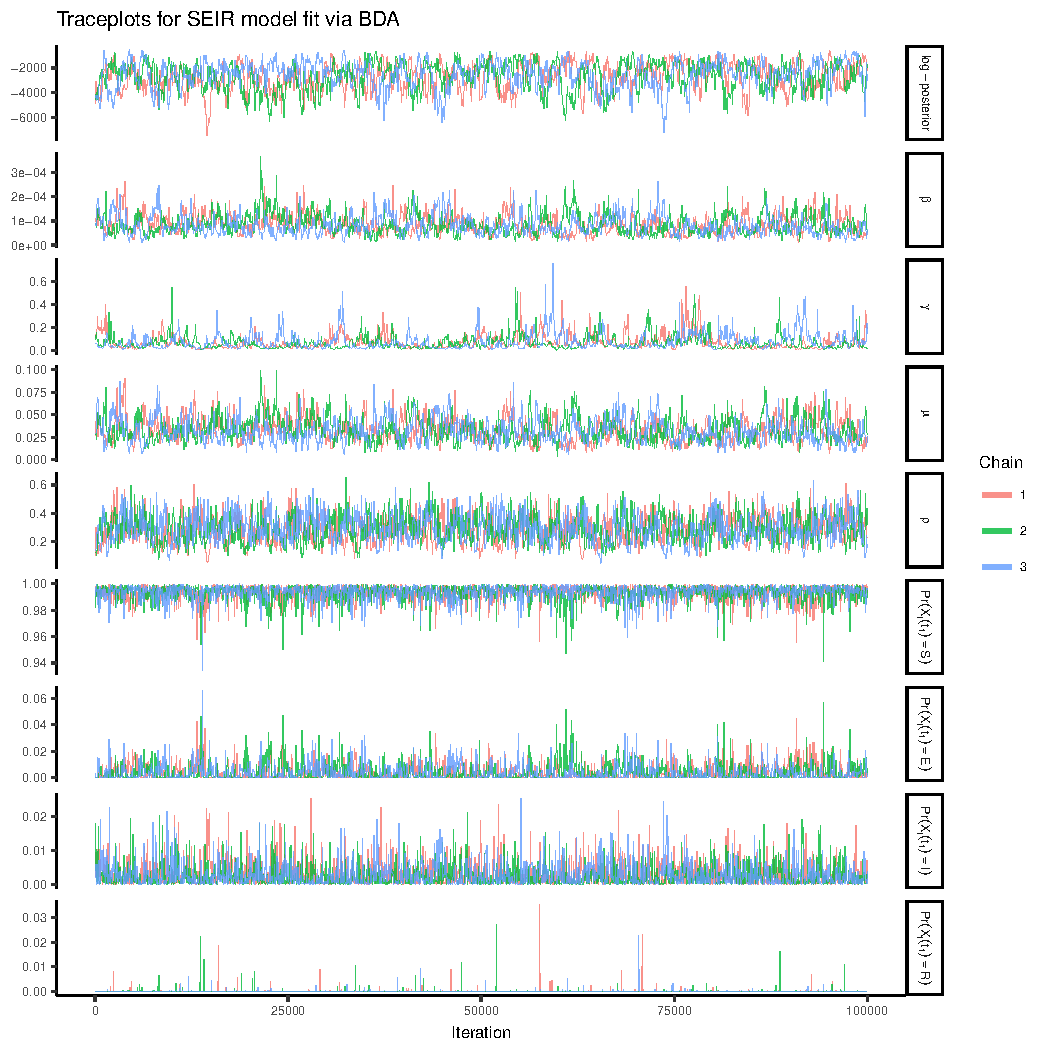
\includegraphics[width=0.9\linewidth]{figures/seir_bda_traceplots}
	\caption[Simulation 1 MCMC traceplots for an SEIR model fit using Bayesian data augmentation.]{Traceplots of the log--posterior and model parameters for the SEIR model fit using Bayesian data augmentation following an initial burn--in of 10 iterations. $ \beta $ denotes the per--contact infectivity rate, $ \gamma $ is the rate at which exposed individuals become infectious, $ \mu $ is the recovery rate, $ \rho $ is the binomial sampling probability. Traceplots are thinned to display every 50\textsuperscript{th} iteration.}
	\label{fig:seirbdatraceplots}
\end{figure}

\begin{figure}[htbp]
	\centering
	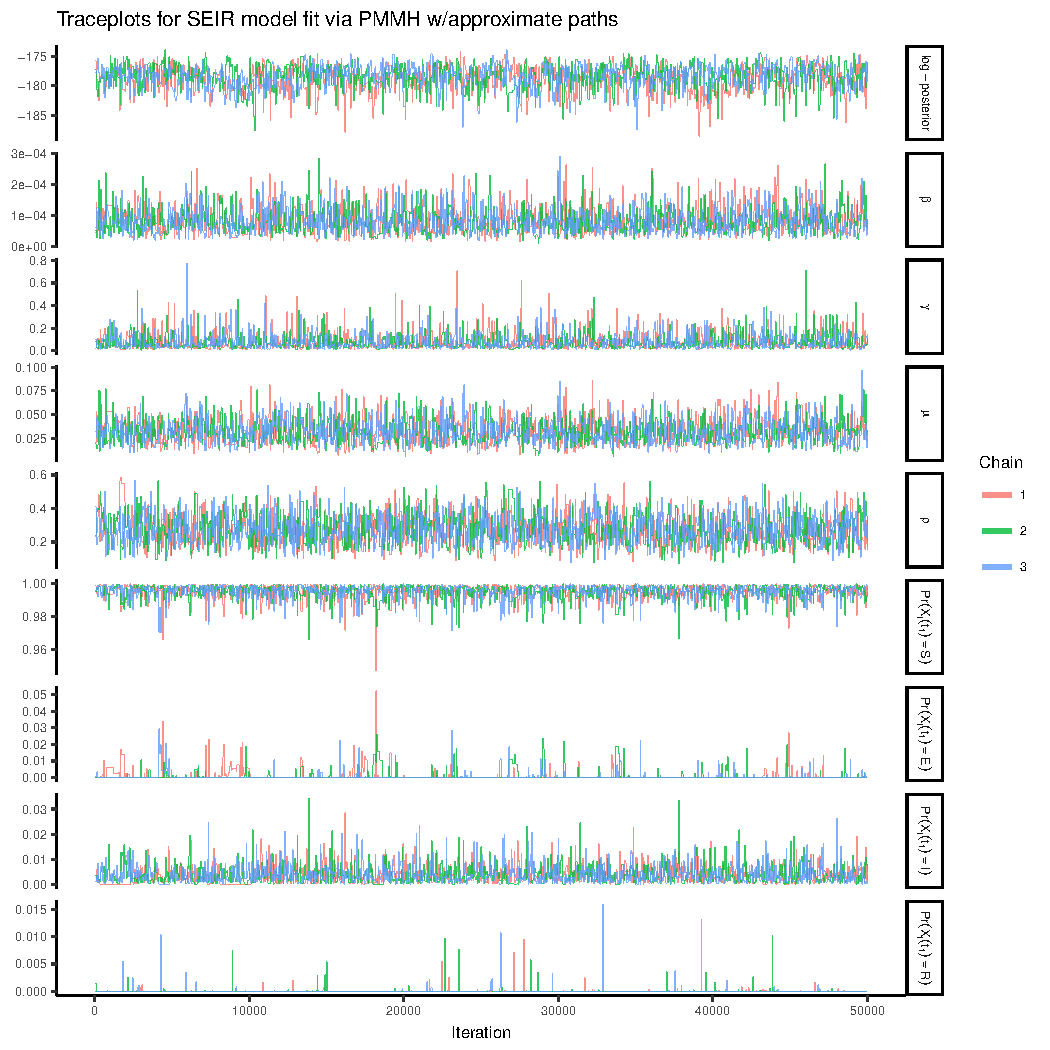
\includegraphics[width=0.9\linewidth]{figures/seir_pomp_approx_traceplots}
	\caption[Simulation 1 MCMC traceplots for an SEIR model fit using PMMH with approximate particle paths.]{Traceplots of the log--posterior and model parameters for the SEIR model fit using PMMH with 200 particles and a time step of 8 hours, following a tuning run of 5,000 iterations used to estimate the covariance matrix for the RWMH and an initial burn--in of 100 iterations. $ \beta $ denotes the per--contact infectivity rate, $ \gamma $ is the rate at which exposed individuals become infectious, $ \mu $ is the recovery rate, $ \rho $ is the binomial sampling probability. Traceplots are thinned to display every 50\textsuperscript{th} iteration.}
	\label{fig:seirpompapproxtraceplots}
\end{figure}

\begin{figure}[htbp]
	\centering
	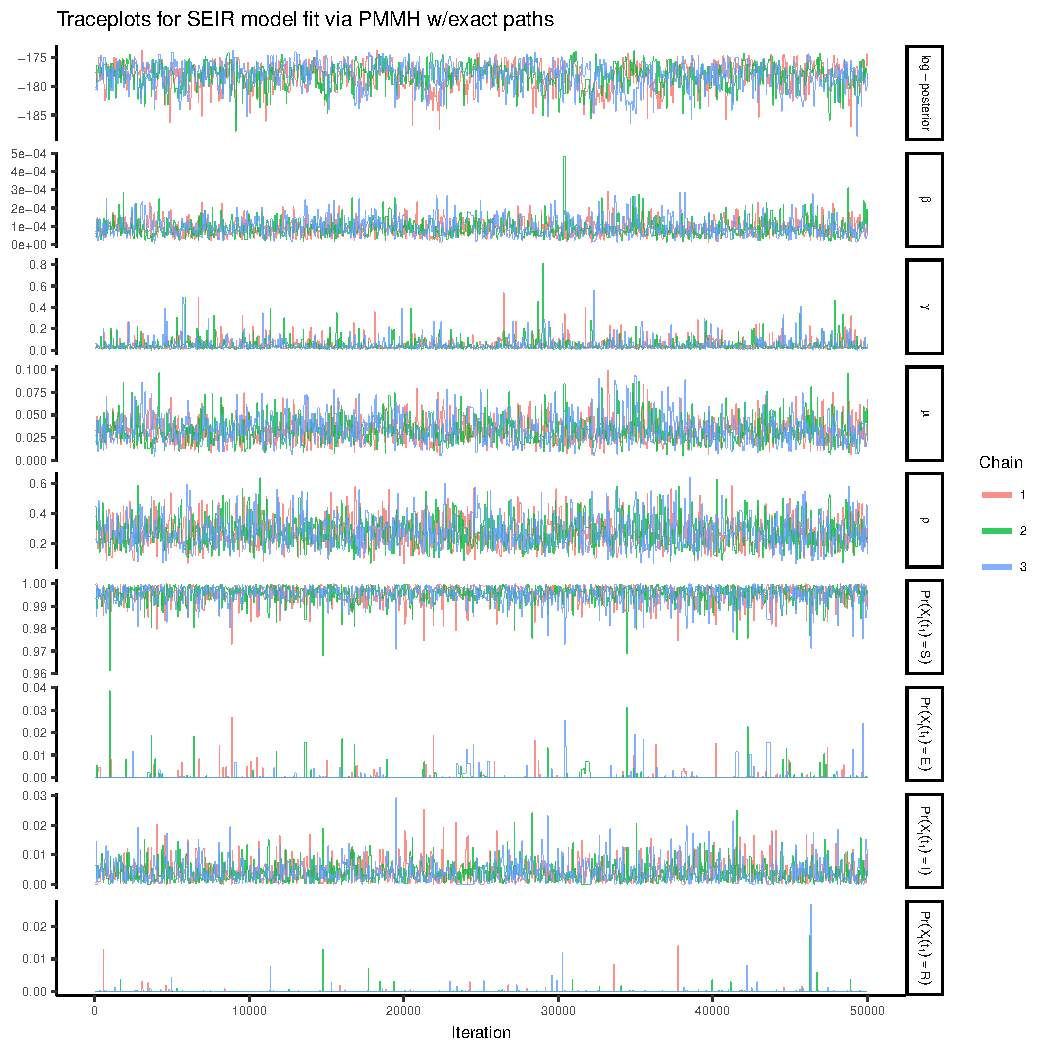
\includegraphics[width=0.9\linewidth]{figures/seir_pomp_exact_traceplots}
	\caption[Simulation 1 MCMC traceplots for an SIR model fit using PMMH with exact particle paths.]{Traceplots of the log--posterior and model parameters for the SIR model fit using PMMH with 200 particles, following a tuning run of 5,000 iterations used to estimate the covariance matrix for the RWMH and an initial burn--in of 100 iterations. $ \beta $ denotes the per--contact infectivity rate, $ \gamma $ is the rate at which exposed individuals become infectious, $ \mu $ is the recovery rate, $ \rho $ is the binomial sampling probability. Traceplots are thinned to display every 50\textsuperscript{th} iteration.}
	\label{fig:seirpompexacttraceplots}
\end{figure}

\newpage
\subsection{Simulation details for the SIRS model}
The final outbreak was simulated under SIRS dynamics in a population of 200 individuals, in which $ R_0 = \beta N / \mu = 2.52 $, the mean infectious period was $ 1/\mu = 14 $ days, and the mean time until loss of immunity was $ 1/\gamma = 150 $ days. One percent of of the population was initially at the time of the first observation and the rest of the individuals were susceptible. Prevalence was observed weekly, with detection probability $ \rho = 0.95 $, over a one year period that spanned the initial wave of the epidemic as well as most of the second wave of the epidemic. 

We ran three chains for 300,000 iterations each, sampling the paths for 3 subjects, chosen uniformly at random, per MCMC iteration. We discarded the first 2,000 iterations from each chain as burn-in. Priors for the rate parameters (summarized in Table \ref{tab:sim1_sirs_priors}) were scaled so that the prior mass spanned a reasonable range of values, but were otherwise mild. Similarly, the prior for the binomial sampling probability reflected a general prior belief that more than 60\% of cases were detected, but was not otherwise particularly informative. The prior for the initial distribution parameters was informative.

\begin{table}[htbp]
	\centering
	\begin{tabular}{lll}
		\hline
		Param. & True Value & Prior distribution \\ 
		\hline
		$ R_0 $ & 2.52 & Beta$ ^\prime $(0.1, 1.5, 1, 28) \\
		$ \beta $ & 0.1 & Gamma$ (0.1, 100) $ \\
		$ \mu $ & 0.036 & Gamma(1.8, 14)  \\ 
		$ \gamma $ & 0.071 & Gamma$ (0.0625, 10) $\\ 
		$ \bp_{t_1} $ & (0.99, 0.01, 0) & Dirichlet(90, 1.5, 0.01)  \\ 
		$ \rho $ & 0.95 & Beta(5, 1) \\
		\hline
	\end{tabular}
	\caption[Simulation 1 SIRS model priors.]{Prior distributions for SIRS model and measurement process parameters. The prior for $ R_0 $ is the induced prior implied by $ \beta $ and $ \mu $. The per--contact infectivity rate is $ \beta $, the recovery rate is $ \mu $, the rate at which immunity is lost is $ \gamma $, the binomial sampling probability is $ \rho $, and the initial state probabilities are $ \bp_{t_1} $.}
	\label{tab:sim1_sirs_priors}
\end{table}

We also fit the SIRS model to the data using PMMH. We ran three MCMC chains with the PMMH algorithm for 50,000 iterations each with 500 particles per chain, and discarded the first 100 iterations as burn-in. We also ran a set of chains with 200 particles but mixing was poor and not all of the chains converged. We attempted to exactly simulate particle paths but ultimately failed due to degeneracies in the algorithm. The time step for the $ \tau $--leaping algorithm was 8 hours. Parameters were updated using random walk Metropolis--Hastings (RWMH) with a proposal covariance matrix estimated from an initial run of 5,000 iterations using an adaptive RWMH algorithm with a target acceptance rate of 23.4\%. We updated parameters on transformed scales in order to remove restrictions on the parameter space, applying a log transformation to $ \beta $, $ \mu $, and $ \gamma $, a logit transformation to $ \rho $, and a generalized logit transformation to $ \bp_{t_1} $.

\newpage
\subsection{Additional results and MCMC diagnostics for the SIRS model}

\begin{table}[htbp]
	\centering
	\begin{tabular}{llrrrr}
		\hline
		Model & Method & Chain & Time & ESS & ESS per CPU time \\ 
		\hline
		SIRS & BDA &  1 & 14.2 & 167.7 & 11.8 \\ 
		SIRS & BDA &  2 & 10.9 & 194.8 & 17.8 \\ 
		SIRS & BDA &  3 & 10.8 & 243.0 & 22.6 \\ 
		SIRS & PMMH - A &  1 & 3.1 & 670.8 & 214.1 \\ 
		SIRS & PMMH - A &  2 & 3.0 & 799.5 & 267.3 \\ 
		SIRS & PMMH - A &  3 & 3.5 & 766.2 & 217.1 \\ 
		SIRS & PMMH - E &  1 & 50.2 & 570.9 & 11.4 \\ 
		SIRS & PMMH - E &  2 & 48.6 & 667.6 & 13.7 \\ 
		SIRS & PMMH - E &  3 & 48.8 & 592.6 & 12.1 \\ 
		\hline
	\end{tabular}
	\caption[Simulation 1 SIRS model run times and log--posterior effective sample sizes.]{Run times, log--posterior effective sample sizes (ESSs), and effective sample sizes per CPU time measure in hours (ESS.per.CPU.time). BDA indicates our Bayesian data augmentation algorithm, PMMH--A indicates PMMH with paths simulated approximately via $ \tau $--leaping algorithm, and PMMH--E indicates PMMH with paths simulated exactly using Gillespie's direct algorithm. The BDA chains were run for 100,000 iterations each, while the PMMH chains were run for 50,000 iterations following a tuning run of 5,000 iterations.}
	\label{tab:sim1_sirs_ess}
\end{table}

\begin{figure}[htbp]
	\centering
	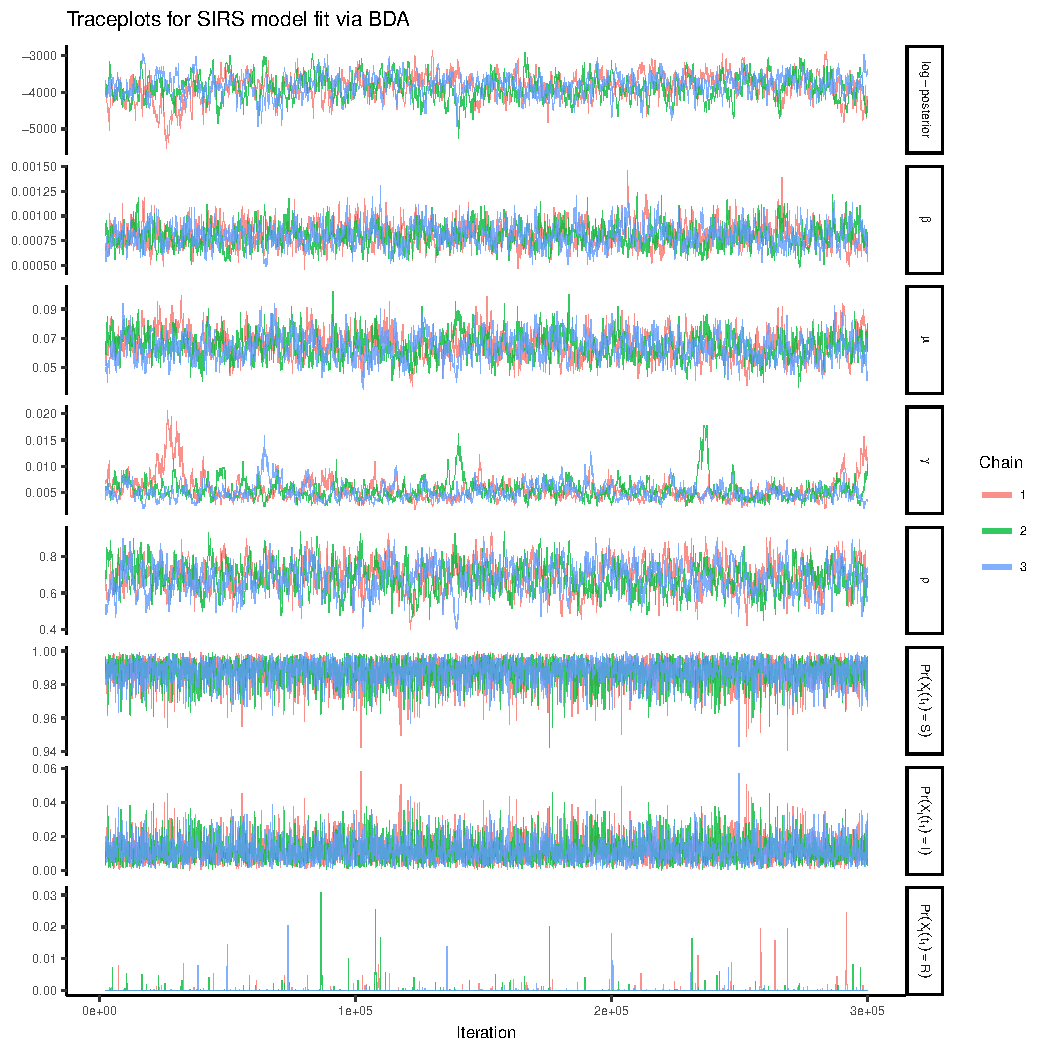
\includegraphics[width=0.9\linewidth]{figures/sirs_bda_traceplots}
	\caption[Simulation 1 MCMC traceplots for an SIR model fit using Bayesian data augmentation.]{Traceplots of the log--posterior and model parameters for the SIR model fit using Bayesian data augmentation following an initial burn--in of 2,000 iterations. $ \beta $ denotes the per--contact infectivity rate, $ \mu $ is the recovery rate, $\gamma$ is the rate at which immunity is lost, and $ \rho $ is the binomial sampling probability. Traceplots are thinned to display every 50\textsuperscript{th} iteration.}
	\label{fig:sirsbdatraceplots}
\end{figure}

\begin{figure}[htbp]
	\centering
	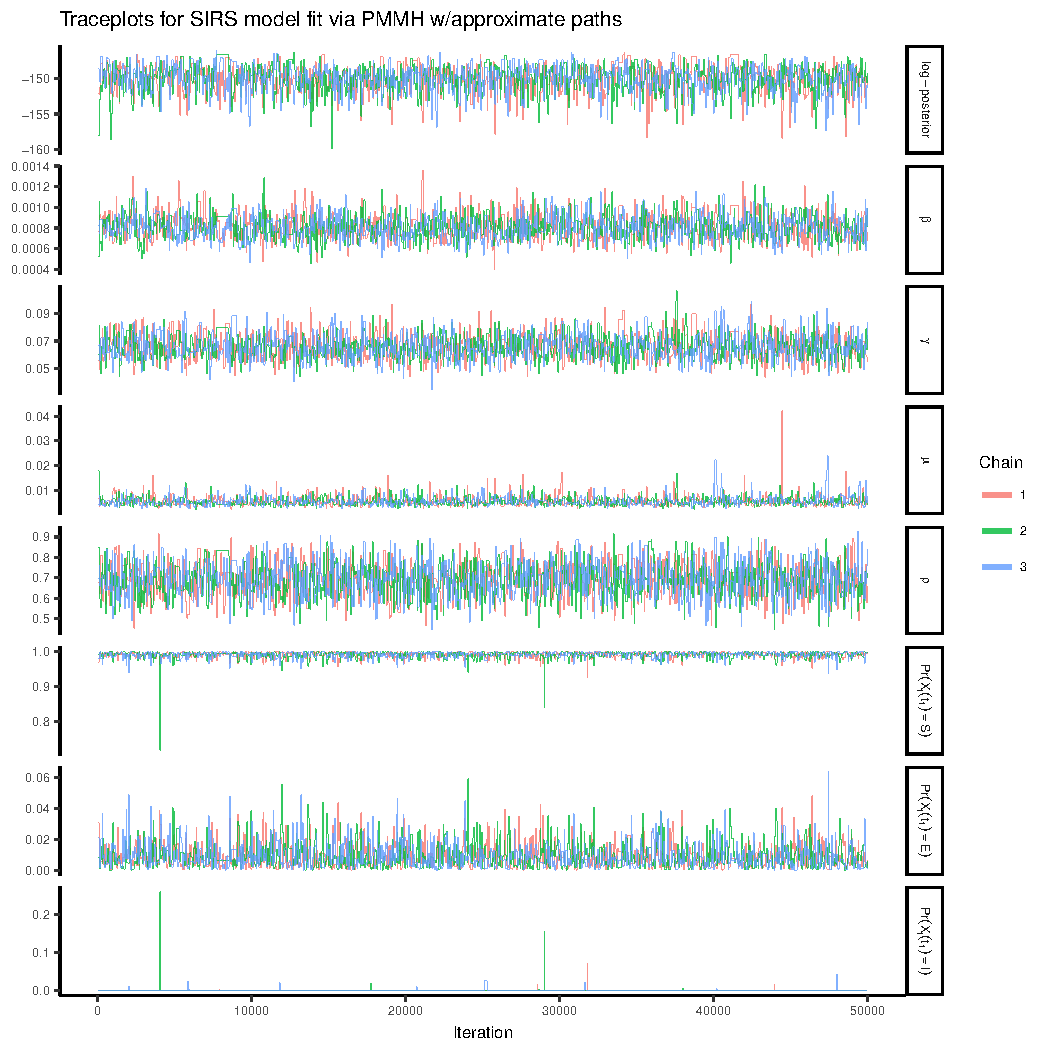
\includegraphics[width=0.9\linewidth]{figures/sirs_pomp_approx_traceplots}
	\caption[Simulation 1 MCMC traceplots for an SIRS model fit using PMMH with approximate particle paths with 500 particles per chain.]{Traceplots of the log--posterior and model parameters for the SIR model fit using PMMH with 500 particles per chain and a time--step of 8 hours in the approximate $ \tau $--leaping algorithm, following a tuning run of 5,000 iterations to estimate the RWMH covariance matrix and in initial burn--in of 100 iterations. $ \beta $ denotes the per--contact infectivity rate, $ \mu $ is the recovery rate, $\gamma$ is the rate at which immunity is lost, and $ \rho $ is the binomial sampling probability. Traceplots are thinned to display every 50\textsuperscript{th} iteration.}
	\label{fig:sirspompapproxtraceplots}
\end{figure}

\begin{figure}[htbp]
	\centering
	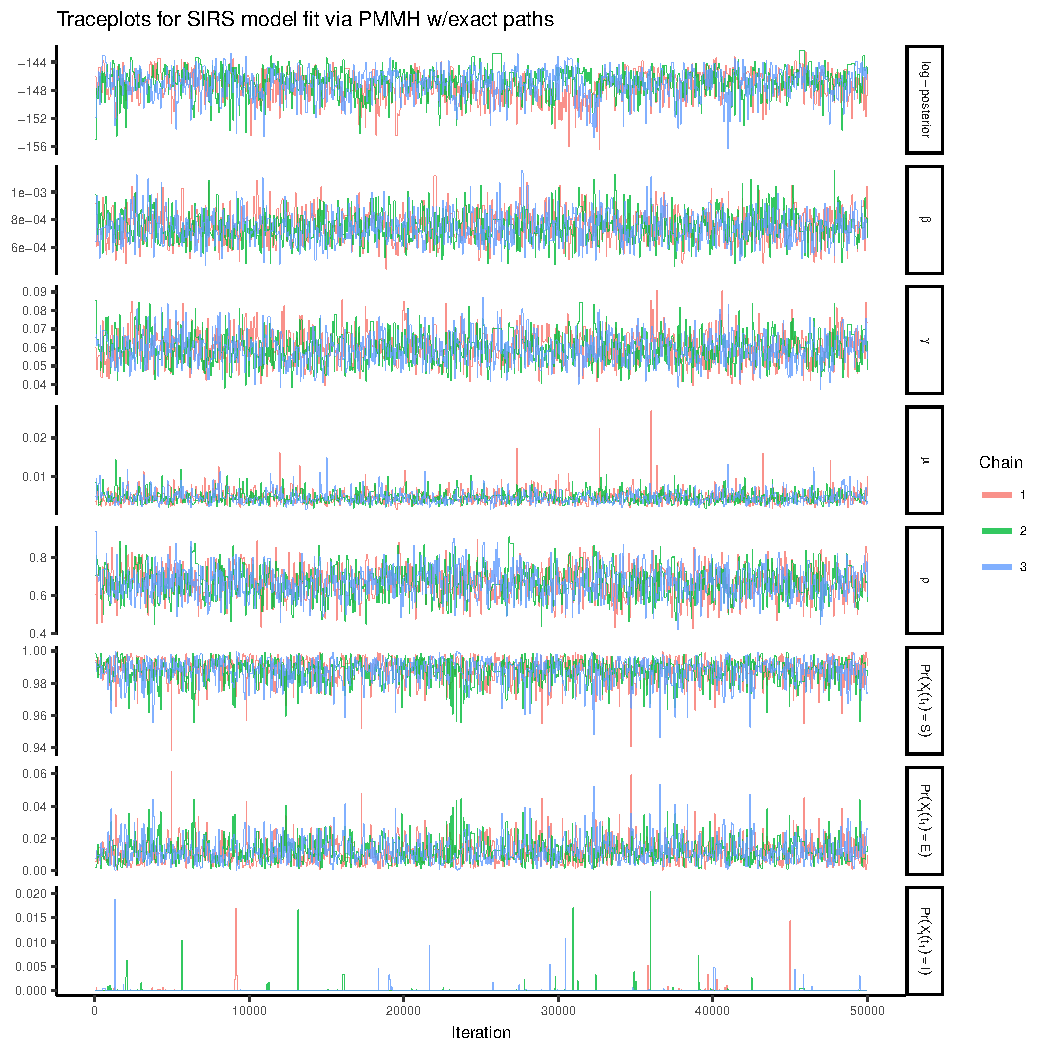
\includegraphics[width=0.9\linewidth]{figures/sirs_pomp_exact_traceplots}
	\caption[Simulation 1 MCMC traceplots for an SIRS model fit using PMMH with exact particle paths with 500 particles per chain.]{Traceplots of the log--posterior and model parameters for the SIR model fit using PMMH with 500 particles per chain and particle paths simulated exactly via Gillespie's direct algorithm, following a tuning run of 5,000 iterations to estimate the RWMH covariance matrix and in initial burn--in of 100 iterations. $ \beta $ denotes the per--contact infectivity rate, $ \mu $ is the recovery rate, $\gamma$ is the rate at which immunity is lost, and $ \rho $ is the binomial sampling probability. Traceplots are thinned to display every 50\textsuperscript{th} iteration.}
	\label{fig:sirspompexacttraceplots}
\end{figure}

\begin{figure}[htbp]
	\centering
	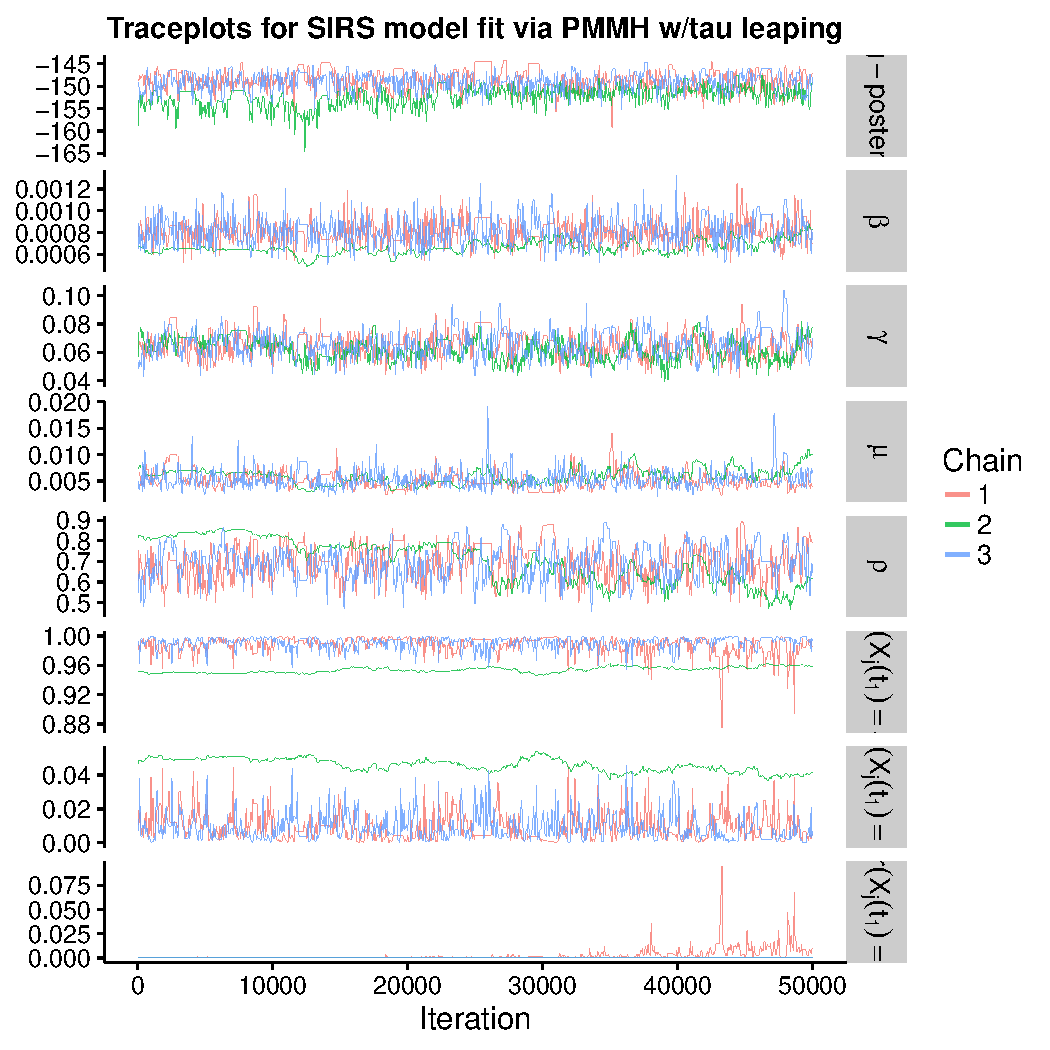
\includegraphics[width=0.9\linewidth]{figures/sirs_pomp_approx_traceplots_np200}
	\caption[Simulation 1 MCMC traceplots for an SIRS model fit using PMMH with exact particle paths with 200 particles per chain.]{Traceplots of the log--posterior and model parameters for the SIR model fit using PMMH with 200 particles per chain and a time--step of 8 hours in the approximate $ \tau $--leaping algorithm, following a tuning run of 5,000 iterations to estimate the RWMH covariance matrix and in initial burn--in of 100 iterations. $ \beta $ denotes the per--contact infectivity rate, $ \mu $ is the recovery rate, $\gamma$ is the rate at which immunity is lost, and $ \rho $ is the binomial sampling probability. Traceplots are thinned to display every 50\textsuperscript{th} iteration.}
	\label{fig:sirspompapproxtraceplotsnp200}
\end{figure}

\newpage
\subsection{Estimated latent posterior distributions for all models}
\begin{figure}[htbp]
	\centering
	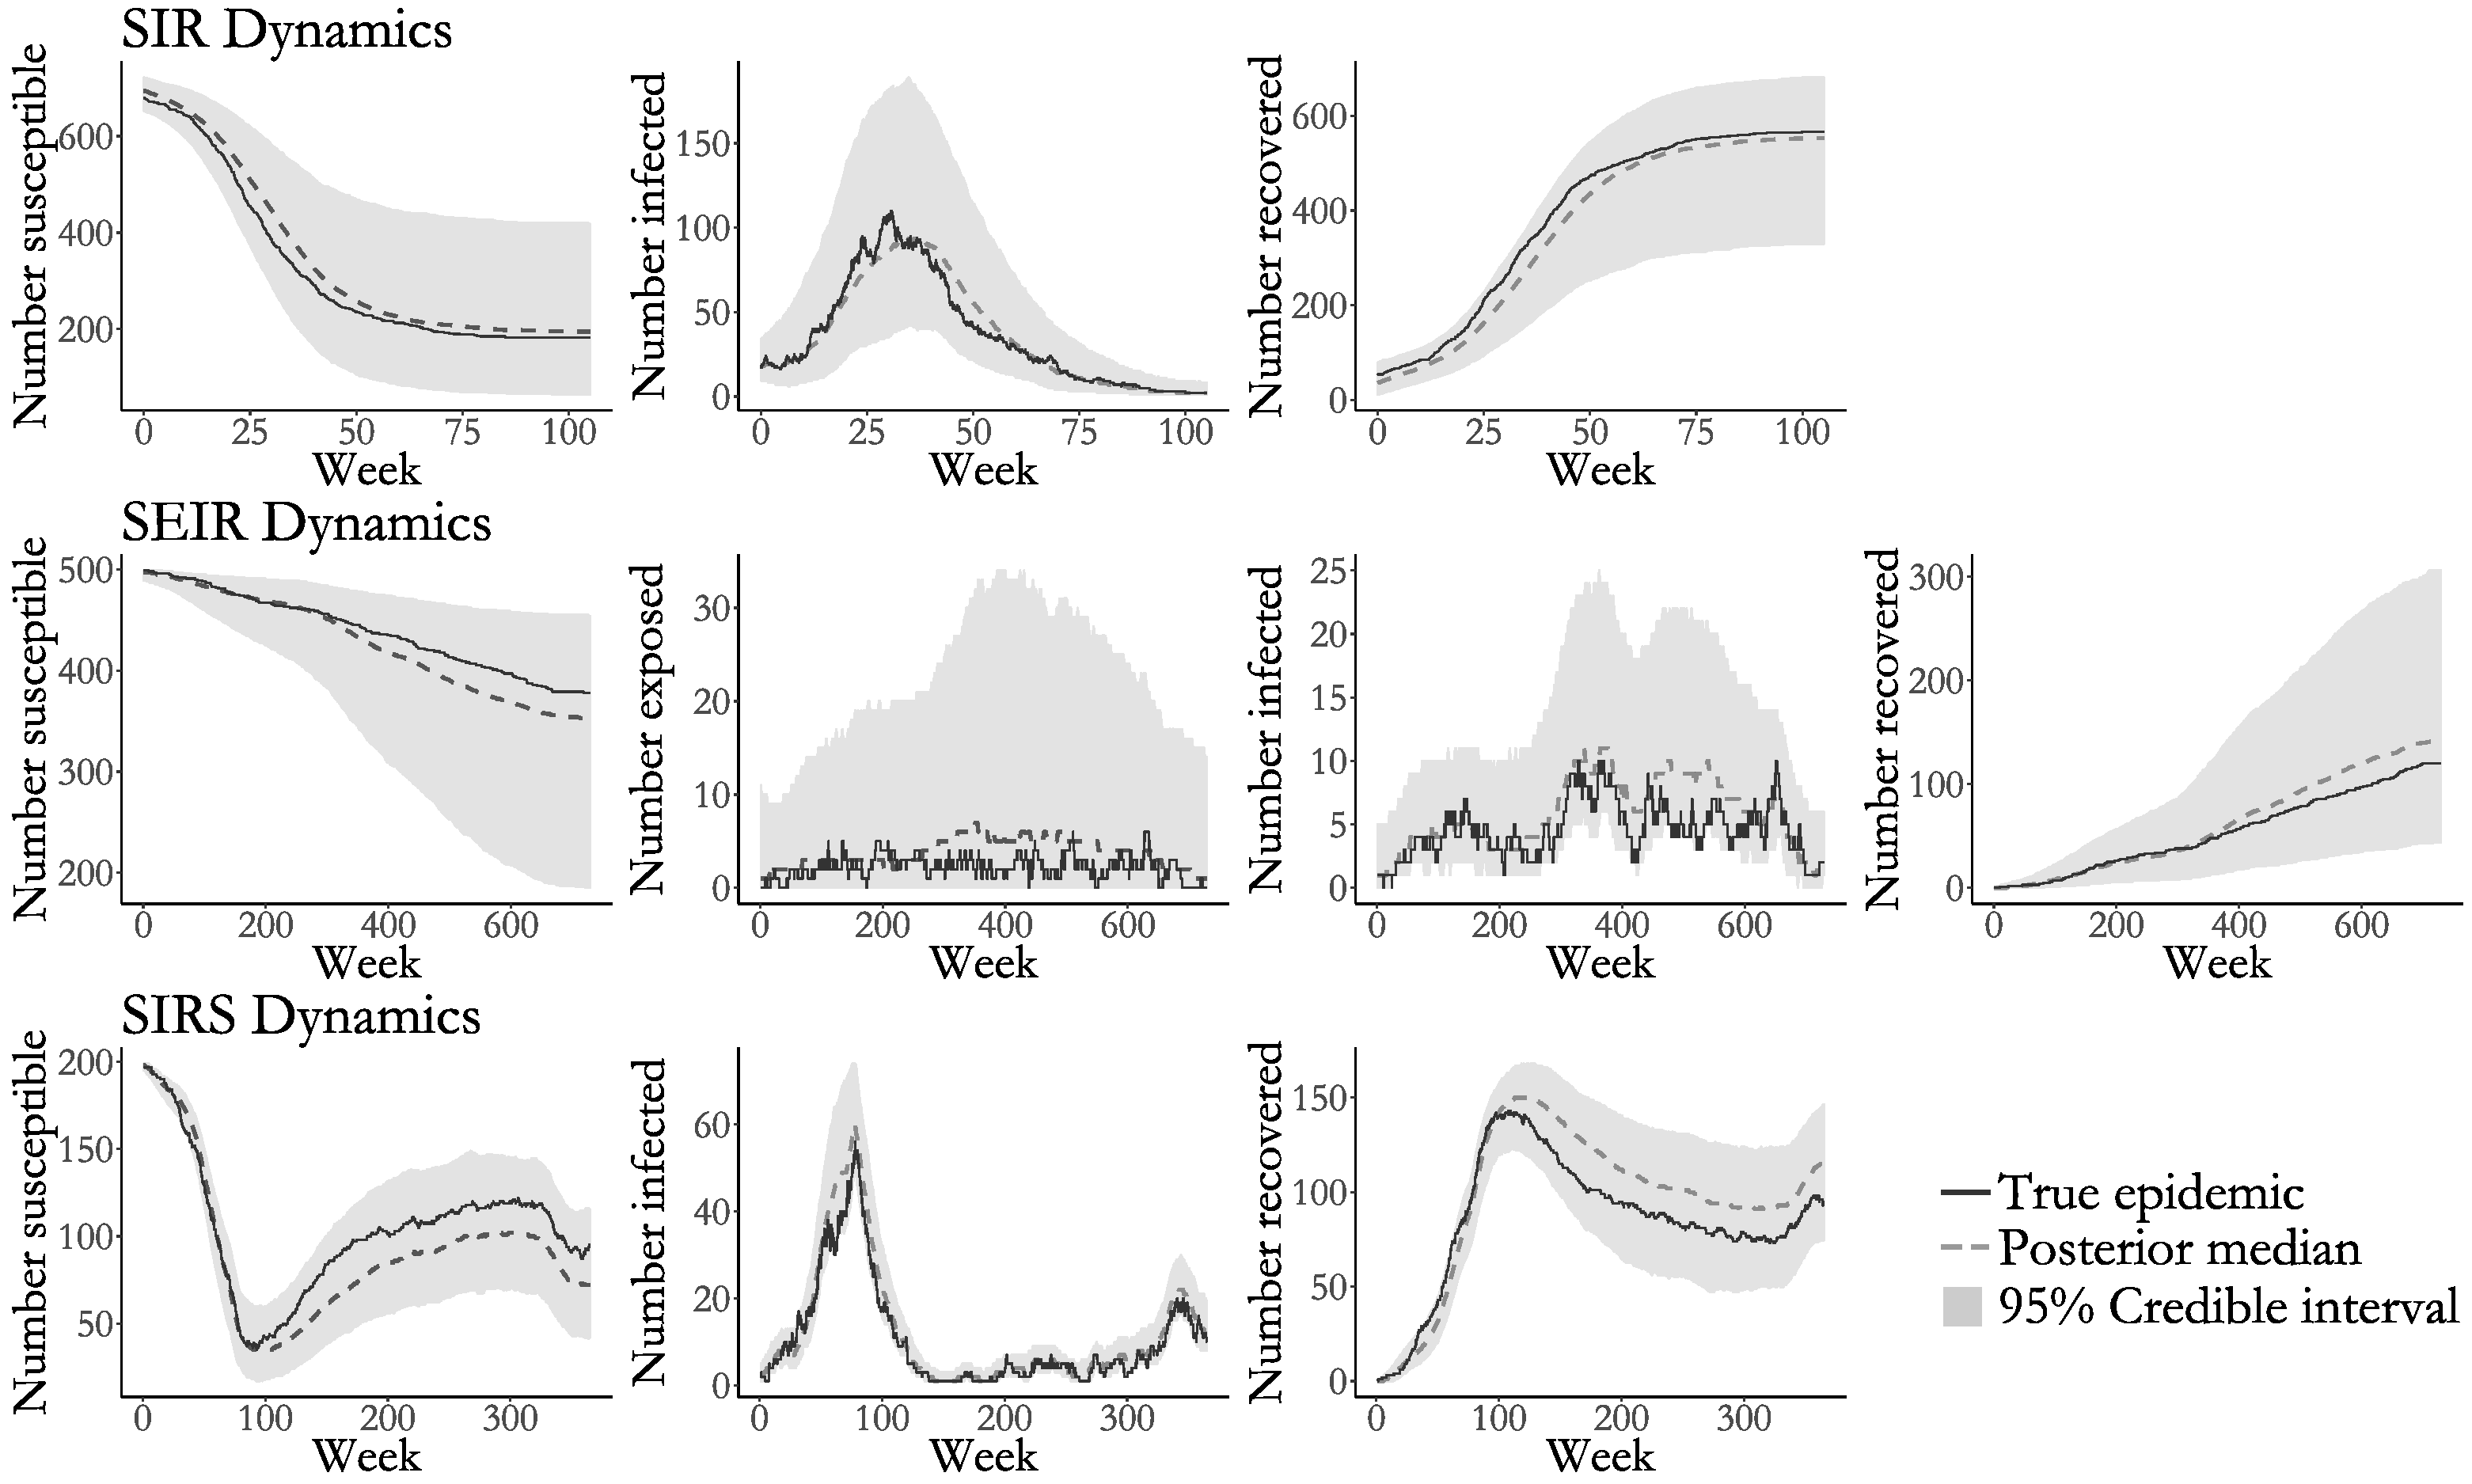
\includegraphics[width=\linewidth]{figures/sim1_latent_posts_all.pdf}
	\caption[Simulation 1 latent posterior distributions for all models.]{Pointwise posterior medians (dashed lines) and pointwise 95\% credible intervals for the numbers of individuals in each disease state for the SIR, SEIR, and SIRS models. True compartment counts are shown as solid lines. Estimates are based on a thinned sample, retaining the collection of disease histories at the end of every 250$ ^{th} $ MCMC iteration.}
	\label{fig:sim1_latent_post_all}
\end{figure}

\newpage
\section{Simulation 2 --- Inference under Model Misspecification,\\ Setup and Additional Results}
\label{sec:bda_misspec_sim_details}
\subsection{Simulation setup}
We simulated an epidemic in a population of size N=400 with time--varying dynamics using Gillespie's direct algorithm over a four year period. Weekly prevalence counts were binomially distributed with detection probability $ \rho = 0.95 $. The epidemic dynamics varied over four epochs, based on the parameters given in Table \ref{tab:misspec_sim_params}. We fit SIR and SEIR models to the data, running three MCMC chains per model, discarding the first 100 iterations as burn--in, and sampling the paths of 150 subjects, chosen uniformly at random, per MCMC iteration. After discarding the burn--in, the resulting samples were combined to form the final sample. We also attempted to fit the models using PMMH. We ran three chains per model, each using 2,500 particles, the paths for which were simulated approximately via $ \tau$--leaping with a one day time step. The PMMH chains were plagued by severe particle degeneracy and did not converge.

\begin{small}
\begin{table}[htbp]
	\centering
	\begin{tabular}{ll}
		\textbf{Epoch 1: Weeks 0 -- 26} & \\
		\hline\hline
		Param. & True value \\ 
		\hline
		$ \beta $ &  0.00025 \\
		$ \gamma $ & 1/210\\
		$ \mu $ &  1/150 \\ 
		$ \rho $ &  0.95 \\
		$ \bX(t_0) $ &  $ S_0 = 397, E_0 = 2, I_0 = 1, R_0 =0 $  \\ 
		\hline	
		\textbf{Epoch 2: Weeks 26--105} & \\
		\hline\hline
		$ \beta $ &  0.0001 \\
		$ \gamma $ & 1/210\\
		$ \mu $ &  1/330 \\ 
		$ \rho $ &  0.95 \\
		$ \bX(t_{26}) $ &  $ S_0 = 279, E_0 = 98, I_0 = 20, R_0 =3 $  \\ 
		\hline
		\textbf{Epoch 3: Weeks 105--167} & \\
		\hline\hline
		$ \beta $ &  0.00035 \\
		$ \gamma $ & 1/90\\
		$ \mu $ &  1/300 \\ 
		$ \rho $ &  0.95 \\
		$ \bX(t_{105}) $ &  $ S_0 = 1, E_0 = 43, I_0 = 145, R_0 =211 $  \\ 
		\hline
		\textbf{Epoch 4: Weeks 167 -- 209} & \\
		\hline\hline
		$ \beta $ &  0.0001 \\
		$ \gamma $ & 1/180\\
		$ \mu $ &  1/70 \\ 
		$ \rho $ &  0.95 \\
		$ \bX(t_{167}) $ &  $ S_0 = 0, E_0 = 1, I_0 = 52, R_0 = 347 $\\
		\hline
	\end{tabular}
	\caption[Simulation 2 SEIR model parameters.]{Parameter values governing the time--varying SEIR dynamics and binomial emissions process. The epidemic was simulated using Gillespie's direct algorithm and the process was restarted with the new parameter values at the beginning of each epoch.}
	\label{tab:misspec_sim_params}
\end{table}
\end{small}

\begin{table}[htbp]
	\centering
	\begin{tabular}{ll}
		\textbf{SIR model} & \\
		\hline\hline
		Parameter & Prior distribution \\ 
		\hline
		$ R_0 $ &  Beta$ ^\prime $(0.6, 0.7, 1, 4) \\
		$ \beta $ &  Gamma$ (0.6, 10000) $ \\
		$ \mu $ &  Gamma(0.7, 100) \\ 
		$ \bp_{t_1} $ &  Dirichlet(90, 0.5, 0.01)  \\ 
		$ \rho $ &  Beta(10, 1) \\
		\hline	
		\textbf{SEIR model} & \\
		\hline\hline
		$ R_0 $ &  Beta$ ^\prime $(0.6, 0.7, 1, 4) \\
		$ \beta $ &  Gamma$ (0.6, 10000) $ \\
		$ \gamma $ &  Gamma$ (0.5, 100) $\\ 
		$ \mu $ &  Gamma(0.7, 100) \\ 
		$ \bp_{t_1} $ &  Dirichlet(90, 0.5, 0.5, 0.01)  \\ 
		$ \rho $ &  Beta(10, 1) \\
		\hline
	\end{tabular}
	\caption[Simulation 2 priors for SIR and SEIR models.]{Prior distributions for the SIR and SEIR model and measurement process parameters for the models fit to the dataset simulated under time--varying SEIR dynamics. The prior for $ R_0 $ is the induced prior implied by $ \beta $ and $ \mu $. The per--contact infectivity rate is $ \beta $, the rate at which an exposed individual becomes infectious is $ \gamma $, the recovery rate is $ \mu $, the binomial sampling probability is $ \rho $, and the initial state probabilities are $ \bp_{t_1} $.}
	\label{tab:misspec_priors}
\end{table}

\newpage
\subsection{Additional results}
\label{subsec:bda_misspec_additional_results}
\begin{table}[htbp]
	\centering
	\begin{tabular}{ll}
		\textbf{SIR model} & \\
		\hline\hline
		Parameter & Posterior median (95\% Credible interval) \\ 
		\hline
		$ R_0 $ & 4.05 (3.40, 4.81) \\ 
		$\beta $ & 0.000035 (0.000030, 0.000040) \\ 
		$ \mu $ & 0.0034 (0.0031, 0.0038) \\ 
		$ \rho $ & 0.95 (0.93, 0.97) \\
		\hline & \\
		\textbf{SEIR model} & \\
		\hline\hline
		Parameter & Posterior median (95\% Credible interval) \\ 
		\hline 
		$ R_0 $ & 23.80 (15.10, 36.98) \\ 
		$ \beta $ & 0.00021 (0.00013, 0.00032) \\ 
		$ \gamma $ & 0.0047 (0.0038, 0.0061) \\ 
		$ \mu $ & 0.0035 (0.0032, 0.0038) \\ 
		$ \rho $ & 0.95 (0.94, 0.97) \\ 
		\hline
	\end{tabular}
	\caption[Simulation 2 posterior estimates for SIR and SEIR model parameters.]{Posterior median estimates and 95\% credible intervals for SIR and SEIR model parameters fit under a binomial emission distribution to the epidemic simulated with time--varying SEIR dynamics.}
\end{table}

\begin{figure}[htbp]
	\centering
	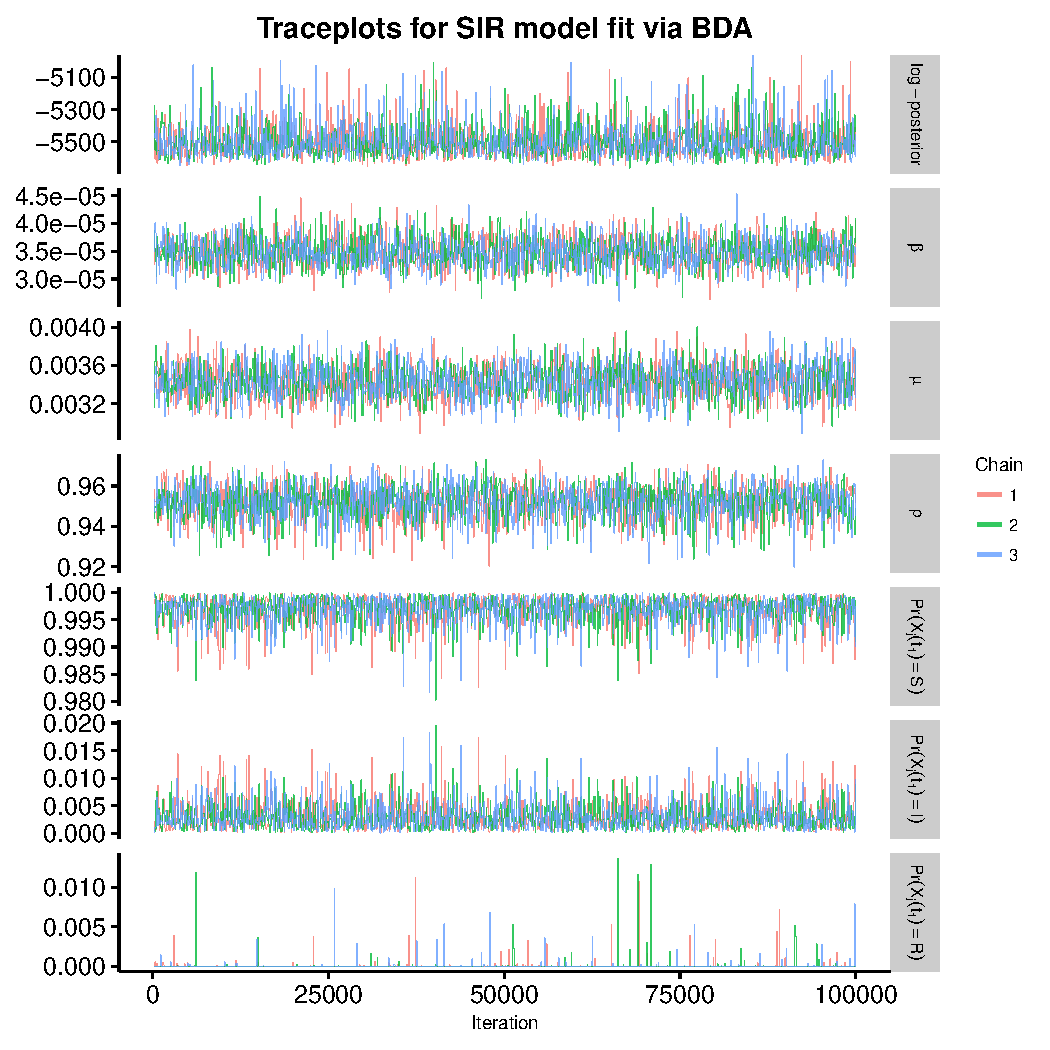
\includegraphics[width=0.9\linewidth]{figures/misspec_sir_bda_traceplots.pdf}
	\caption[Simulation 2 MCMC traceplots for SIR model parameters fit using Bayesian data augmentation.]{Traceplots of the log--posterior and model parameters for the SIR model fit using BDA following an initial burn--in of 100 iterations. $ \beta $ denotes the per--contact infectivity rate, $ \mu $ is the recovery rate, $ \rho $ is the binomial sampling probability. Traceplots are thinned to display every 50\textsuperscript{th} iteration.}
	\label{fig:misspec_sir_bda_traceplots}
\end{figure}

\begin{figure}[htbp]
	\centering
	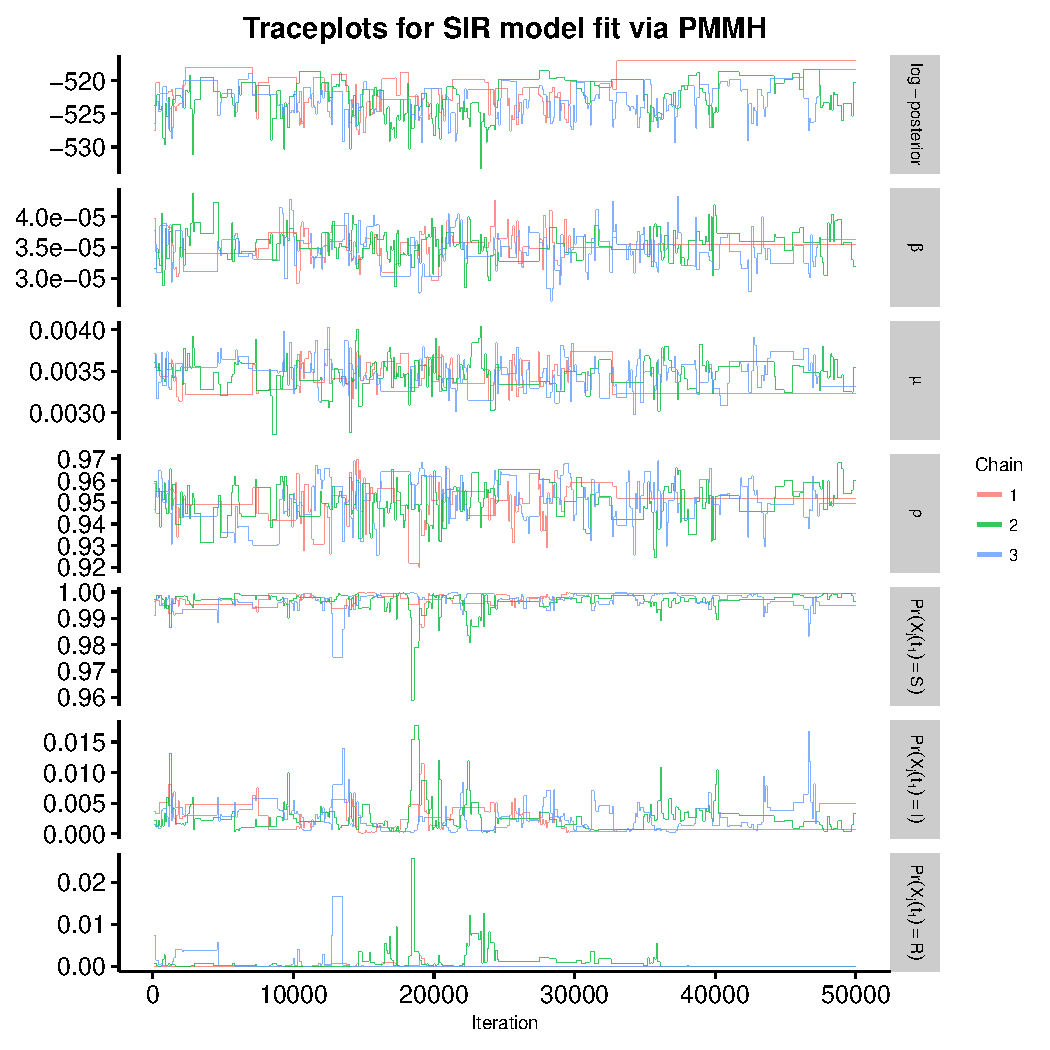
\includegraphics[width=0.9\linewidth]{figures/misspec_sir_pmmh_traceplots.pdf}
	\caption[Simulation 2 MCMC traceplots for SIR model parameters fit using PMMH.]{Traceplots of the log--posterior and model parameters for the SIR model fit using PMMH with 2,500 particles, following a tuning run of 5,000 iterations used to estimate the covariance matrix for the RWMH. $ \beta $ denotes the per--contact infectivity rate, $ \mu $ is the recovery rate, $ \rho $ is the binomial sampling probability. Traceplots are thinned to display every 50\textsuperscript{th} iteration.}
	\label{fig:misspec_sir_pmmh_traceplots}
\end{figure}

\begin{figure}[htbp]
	\centering
	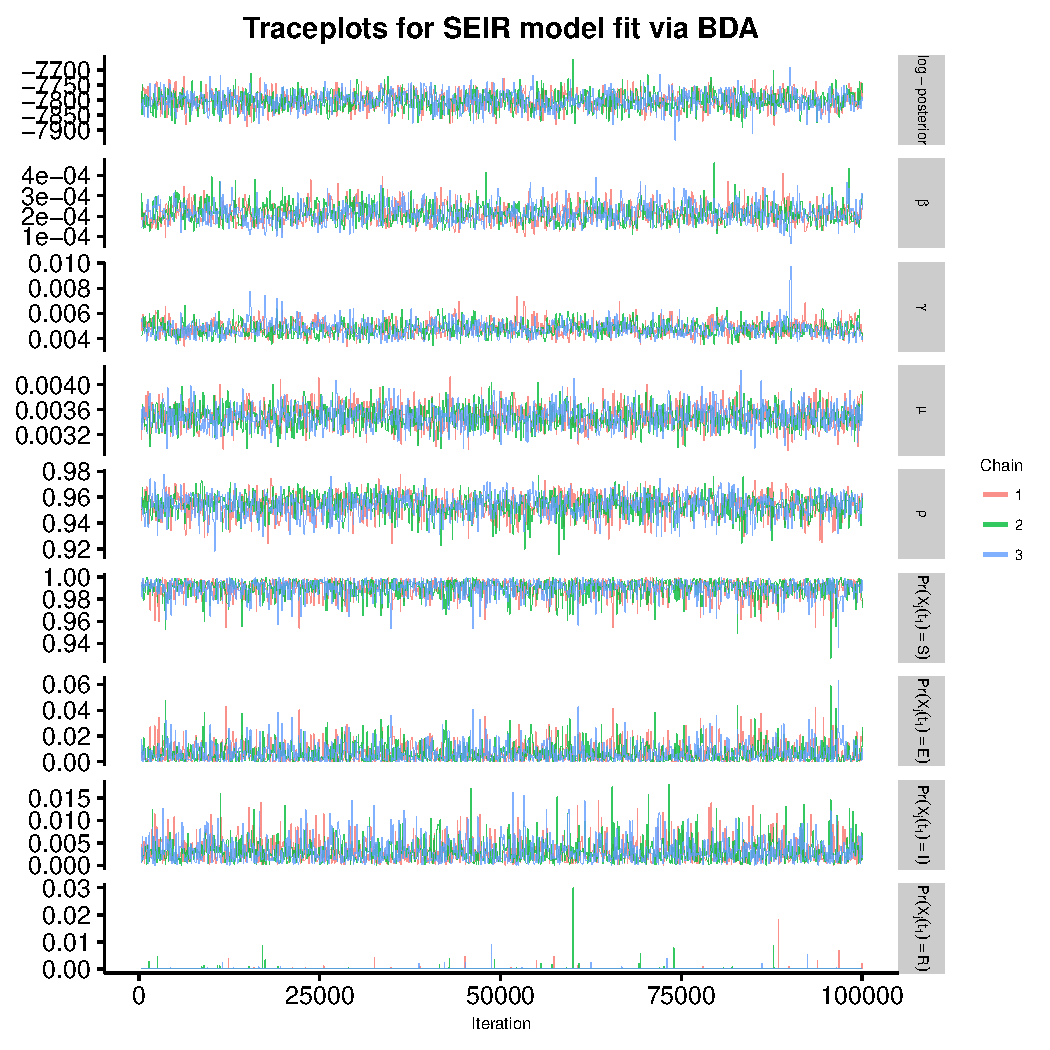
\includegraphics[width=0.9\linewidth]{figures/misspec_seir_bda_traceplots.pdf}
	\caption[Simulation 2 MCMC traceplots for SEIR model parameters fit using Bayesian data augmentation.]{Traceplots of the log--posterior and model parameters for the SEIR model fit using BDA following an initial burn--in of 100 iterations. $ \beta $ denotes the per--contact infectivity rate, $ \gamma $ is the rate at which an exposed individual becomes infectious, $ \mu $ is the recovery rate, $ \rho $ is the binomial sampling probability. Traceplots are thinned to display every 50\textsuperscript{th} iteration.}
	\label{fig:misspec_seir_bda_traceplots}
\end{figure}

\begin{figure}[htbp]
	\centering
	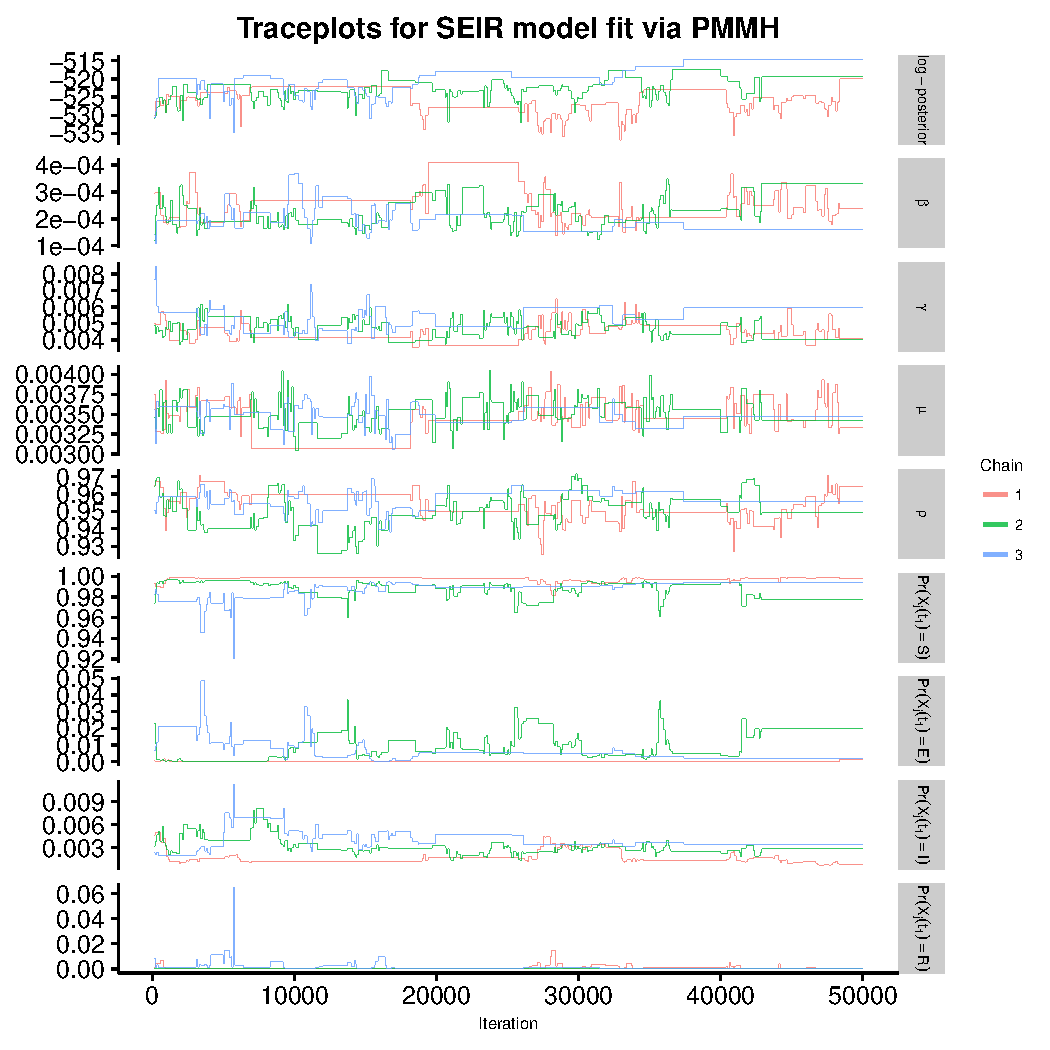
\includegraphics[width=0.9\linewidth]{figures/misspec_seir_pmmh_traceplots.pdf}
	\caption[Simulation 2 MCMC traceplots for SEIR model parameters fit using PMMH.]{Traceplots of the log--posterior and model parameters for the SEIR model fit using PMMH with 2,500 particles, following a tuning run of 5,000 iterations used to estimate the covariance matrix for the RWMH. $ \beta $ denotes the per--contact infectivity rate,  $ \gamma $ is the rate at which an exposed individual becomes infectious, $ \mu $ is the recovery rate, $ \rho $ is the binomial sampling probability. Traceplots are thinned to display every 50\textsuperscript{th} iteration.}
	\label{fig:misspec_seir_pmmh_traceplots}
\end{figure}

\newpage

\section{Simulation 3 --- Inference under Population Size\\ Misspecification --- Details}
\label{sec:popsize_misspec_details}
We simulated an outbreak under SIR dynamics, with $ R_0 = \beta N / \mu =3.5 $, in a population of 1,250 individuals. Roughly 0.2\% of the population was initially infected, and 95\% were initially susceptible. The mean infectious period was $ 1/\mu = 7 $ days. Prevalence was observed at weekly intervals, with detection probability $ \rho = 0.3 $, over a one year period.

We ran three chains for 100,000 iterations each under the following assumed population sized: 150, 300, 500, 900, 1100, 1200, 1250, 1300, 1400. We sampled the paths for 10\% of the subjects, chosen uniformly at random, per MCMC iteration. We discarded the first 500 iterations from each chain as burn-in. Diffuse priors were specified for all model parameters, with the prior for the per--contact infectivity rate depending on the assumed population size (summarized in Table \ref{tab:popsize_misspec_priors}).

\begin{table}[htbp]
	\centering
	\begin{tabular}{ll}
		\hline
		Param. & Prior distribution \\ 
		\hline
		$ R_0 $ &  Beta$ ^\prime $($ 0.00042 \times \frac{1250}{N} $, 0.35, 1, 2 / N) \\
		$ \beta $ &  Gamma$ (0.00042 \times \frac{1250}{N}, 1) $ \\ 
		$ \mu $ & Gamma(0.35, 2)  \\ 
		$ \bp_{t_1} $ & Dirichlet(100, 1, 5)  \\ 
		$ \rho $ & Beta(1,1) \\
		\hline
	\end{tabular}
	\caption[Simulation 3 SIR model priors.]{Prior distributions for SIR model and measurement process parameters. The prior for $ R_0 $ is the induced prior implied by $ \beta $ and $ \mu $. The per--contact infectivity rate is $ \beta $, the recovery rate is $ \mu $, the binomial sampling probability is $ \rho $, and the initial state probabilities are $ \bp_{t_1} $. The prior for $ \beta $ was scaled in accordance with the assumed population size.}
	\label{tab:popsize_misspec_priors}
\end{table}

\newpage

\section{Simulation 4 --- Effect of Prior Specification on\\ Inference --- Setup and Additional Results}
\label{sec:prior_effect_details}
\subsection{Simulation details}
We ran three MCMC chains for each of the SIR models fit under the prior regimes that are specified in Table \ref{tab:prior_effect_priors} along with the true parameter values under which the data were simulated. Each chain was run for 100,000 MCMC iterations  with 75 subject--paths per iteration. The first 100 iterations of each were discarded as burn--in, after which the samples from all three chains for each model were combined to form the posterior sample.

\begin{table}[htbp]
	\centering	
	\footnotesize
	\begin{tabular}{lcccc}
		\hline & \multicolumn{4}{c}{Prior Distribution} \\
		\hline
		Parameter & Regime 1 & Regime 2 & Regime 3 & Regime 4\\
		\hline
		$R_0 = 1.84$ & Beta$ ^\prime $(3, 3, 1, 1.526) & Beta$ ^\prime $(0.3, 0.1, 1, 0.6) & Beta$ ^\prime $(3, 3, 1, 1.526) & Beta$ ^\prime $(0.3, 0.1, 1, 0.6) \\
		$\beta = 0.00035$ & Gamma(3, 10000) & Gamma(0.3, 1000) & Gamma(3, 10000)& Gamma(0.3, 1000) \\
		$\mu = 0.14$ & Gamma(3, 20) & Gamma(0.1, 0.8) & Gamma(3, 20)& Gamma(0.1, 0.8)  \\
		$\rho = 0.2$ & Beta(21, 75) & Beta(21, 75) & Beta(1,1) & Beta(1,1)\\
		\hline 
	\end{tabular} 
	\caption[Simulation 4 prior regimes.]{True parameter values and prior distributions under four different prior regimes. The prior for $ R_0 $ is the implied prior induced by the priors for $ \beta $ and $ \mu $. In regimes one and three, the central 80\% of the prior mass for $ R_0 $ lay between 1.25 and 4.56, while in regimes two and four, 80\% of the prior mass lay between $ 3.8\times10^{-4} $ and $ 2.7\times 10^4 $. In regimes one and two, 80\% of the prior mass for $ \rho $ lay between 0.17 and 0.27, while in regimes three and four the prior mass for $ \rho $ was uniformly distributed between 0 and 1. We used the same mildly informative Dirichlet(9, 0.2, 0.5) prior for $ \bp_{t_1} $ in all prior regimes.}
	\label{tab:prior_effect_priors}
\end{table}

\subsection{Convergence diagnostics}
\begin{figure}[htbp]
	\centering
	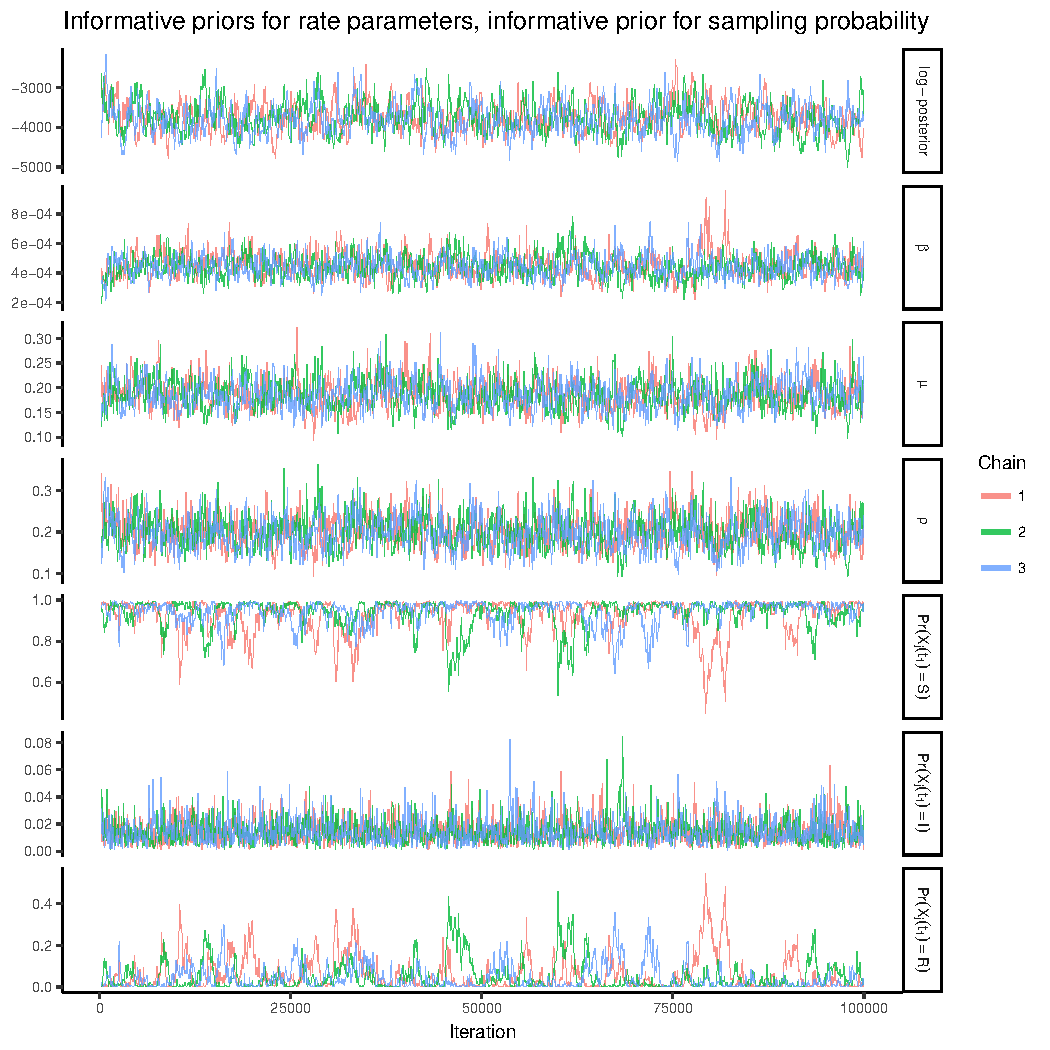
\includegraphics[width=0.9\linewidth]{figures/informative_informative_traceplots.pdf}
	\caption[Simuation 4 MCMC traceplots for SIR model parameters fit under informative priors for all parameters.]{Traceplots of the log--posterior and model parameters for the SIR model fit under informative priors for all model parameters. $ \beta $ denotes the per--contact infectivity rate, $ \mu $ is the recovery rate, $ \rho $ is the binomial sampling probability. Traceplots are thinned to display every 50\textsuperscript{th} iteration.}
	\label{fig:inform_inform_traces}
\end{figure}

\begin{figure}[htbp]
	\centering
	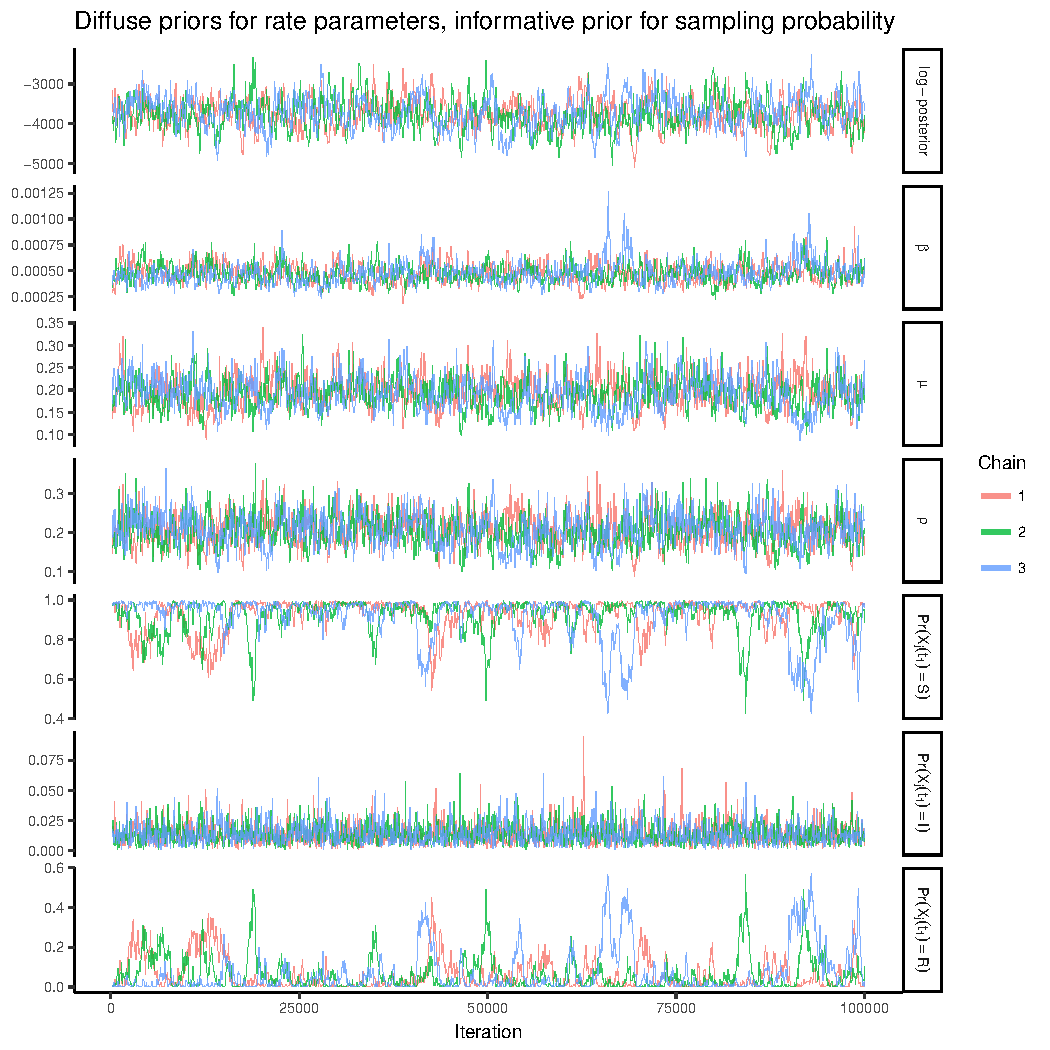
\includegraphics[width=0.9\linewidth]{figures/diffuse_informative_traceplots.pdf}
	\caption[Simuation 4 MCMC traceplots for SIR model parameters fit under informative priors for the measurement process and diffuse priors for rate parameters.]{Traceplots of the log--posterior and model parameters for the SIR model fit under diffuse priors for the rate parameters and an informative prior for the binomial sampling probability. $ \beta $ denotes the per--contact infectivity rate, $ \mu $ is the recovery rate, $ \rho $ is the binomial sampling probability. Traceplots are thinned to display every 50\textsuperscript{th} iteration.}
	\label{fig:diffuse_inform_traces}
\end{figure}

\begin{figure}[htbp]
	\centering
	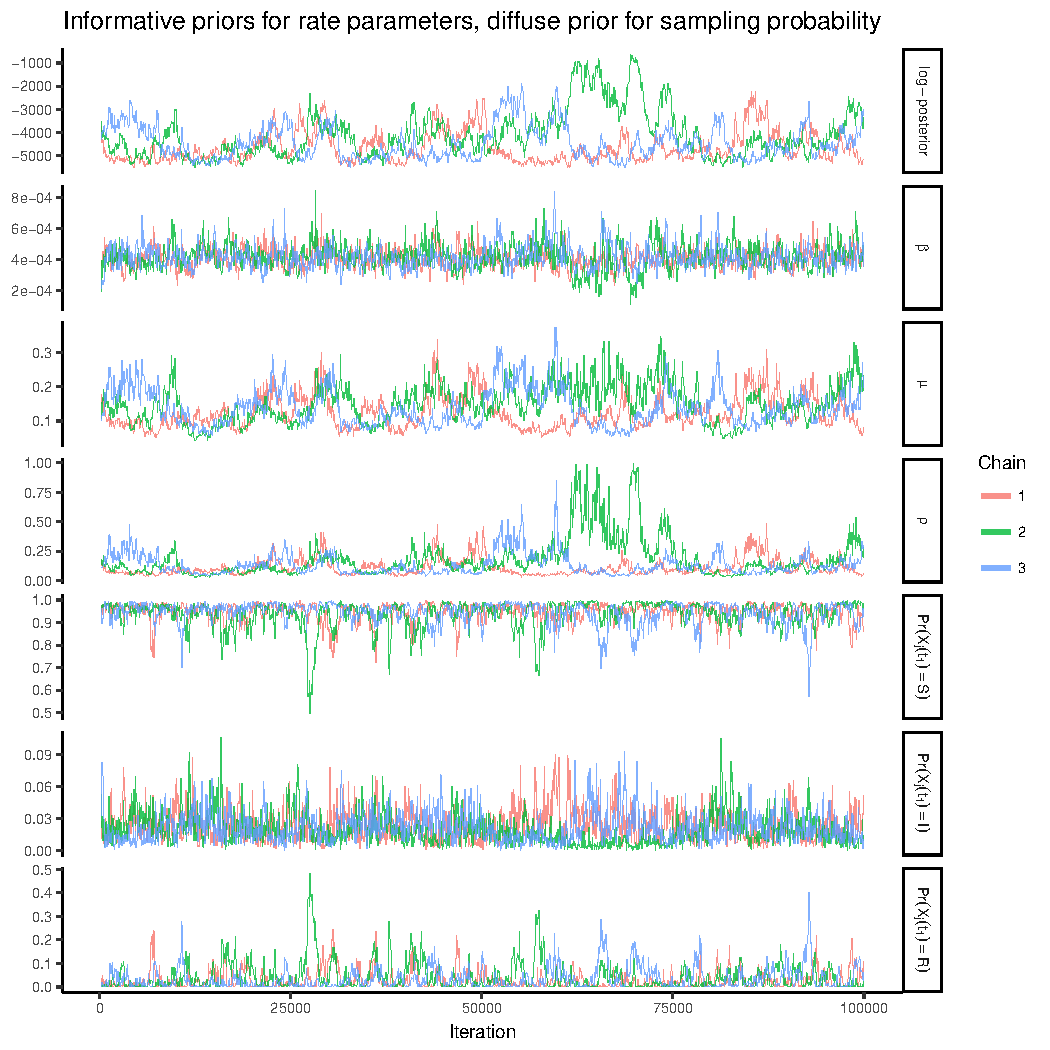
\includegraphics[width=0.9\linewidth]{figures/informative_diffuse_traceplots.pdf}
	\caption[Simuation 4 MCMC traceplots for SIR model parameters fit under diffuse priors for the measurement process and informative priors for rate parameters.]{Traceplots of the log--posterior and model parameters for the SIR model fit under informative priors for the rate parameters and a diffuse prior for the binomial sampling probability. $ \beta $ denotes the per--contact infectivity rate, $ \mu $ is the recovery rate, $ \rho $ is the binomial sampling probability. Traceplots are thinned to display every 50\textsuperscript{th} iteration.}
	\label{fig:inform_diffuse_traces}
\end{figure}

\begin{figure}[htbp]
	\centering
	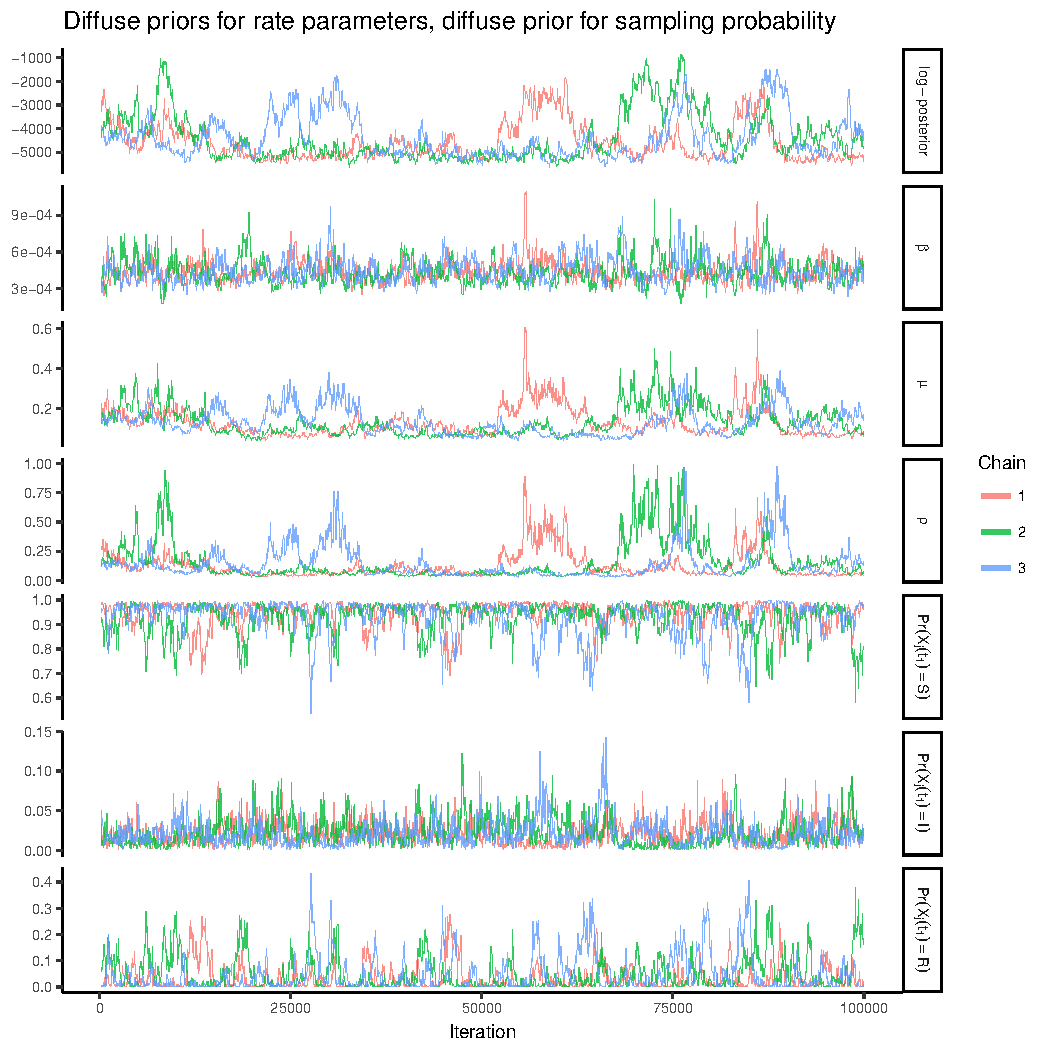
\includegraphics[width=0.9\linewidth]{figures/diffuse_diffuse_traceplots.pdf}
	\caption[Simuation 4 MCMC traceplots for SIR model parameters fit under diffuse priors for the measurement process and diffuse priors for rate parameters.]{Traceplots of the log--posterior and model parameters for the SIR model fit under diffuse priors for all model parameters. $ \beta $ denotes the per--contact infectivity rate, $ \mu $ is the recovery rate, $ \rho $ is the binomial sampling probability. Traceplots are thinned to display every 50\textsuperscript{th} iteration.}
	\label{fig:diffuse_diffuse_traces}
\end{figure}

\newpage
\section{Setup, additional results, and MCMC diagnostics for British boarding school example}
\label{sec:bbs_supp}

We ran three MCMC chains per model to fit the SIR and SEIR models to the British boarding school dataset, for 100,000 iterations per chain. We sampled the paths for 100 subjects, chosen uniformly at random, per MCMC iteration, and discarded, as burn-in, the first 100 iterations of each chain for the SIR model, and the first 5,000 iterations of each chain for the SEIR model. Prior distributions, along with posterior medians and credible intervals are given in tables \ref{tab:bbs_SIR_prior_binom} and \ref{tab:bbs_SEIR_prior_binom}. The induced prior for $ R_0 $ is highly diffuse due to the diffuse prior on the per--contact infectivity rate. The prior distribution for the recovery rate and the rate at which exposed individuals became infectious reflected prior knowledge of the natural history of influenza. The prior for the detection probability has roughly 90\% of its mass above 0.3, but is arguably quite diffuse given that it is known that over 90\% of the boys were eventually infected. 

We also fit the SIR and SEIR models using PMMH with paths for 5,000 particles simulated approximately via a multinomial modification of $ \tau $--leaping over two hour increments. The same priors were used as for the chains fit using BDA. Parameters were updated via random walk Metropolis--Hastings on transformed scales with a proposal covariance matrix that was estimated from an initial run of 2,000 MCMC iterations. We applied a log transformation to the rate parameters, a logit transformation to the binomial sampling probability, and a generalized logit transformation to the initial state probabilities. Results for PMMH are not reported since the MCMC never converged (see traceplots below).

\begin{table}[htbp]
	\begin{center}
		\begin{tabular}{ccc}
			\hline Parameter &  Prior Distribution & Posterior Median (95\% BCI)  \\ 
			\hline
			\hline $R_0$ & Beta$ ^\prime $(0.001, 1, 1, 1526) & 3.89 (3.40, 4.47) \\
			\hline $\beta$ & Gamma(0.001, 1) & 0.0024 (0.0021, 0.0026) \\ 
			\hline $\mu$ & Gamma(1,2) & 0.46 (0.42, 0.50) \\ 
			\hline $\rho $ & Beta(1,2) & 0.98 (0.92, 1.00)\\
			\hline $\Pr(X_j(t_1) = S)$& \multirow{3}{*}{Dirichlet(900,3,9)} & 0.99 (0.98, 0.99) \\
			$\Pr(X_j(t_1) = I)$& & 0.003 (0.001, 0.007) \\
			$\Pr(X_j(t_1) = R)$&  & 0.009 (0.004, 0.017)\\
			\hline 
		\end{tabular} 
		\caption[Prior distributions for an SIR model fit to the British boarding school outbreak data.]{Prior distributions and posterior estimates for parameters of the SIR model with binomial emissions fit to the British boarding school outbreak data. The per--contact infectivity rate is $ \beta $, the recovery rate is $ \mu $, and the binomial sampling probability is $ \rho $. The prior for $ R_0 $ is the implied prior induced by the priors for $ \beta $ and $ \mu $. Effective sample size were $\beta$: 11,304; $\mu$: 16,238; $\rho$: 3,920; $p_{S_{t_1}}$: 26,989; $p_{I_{t_1}}$: 284,431; $p_{R_{t_1}}$: 22,761.}
		\label{tab:bbs_SIR_prior_binom}
	\end{center}
\end{table}

\begin{table}[htbp]
	\begin{center}
		\begin{tabular}{ccc}
			\hline Parameter &  Prior Distribution & Posterior Median (95\% BCI)  \\ 
			\hline
			\hline $R_0$ & Beta$ ^\prime $(0.001, 1, 1, 1526) & 3.89 (3.40, 4.47) \\
			\hline $\beta$ & Gamma(0.001, 1) & 0.0064 (0.0046, 0.0086) \\ 
			\hline $ \gamma $ & Gamma(0.001, 1) & 0.84 (0.66, 1.19) \\
			\hline $\mu$ & Gamma(1,2) & 0.47 (0.43, 0.51) \\ 
			\hline $\rho $ & Beta(1,2) & 0.98 (0.91, 1.00)\\
			\hline $\Pr(X_j(t_1) = S)$& \multirow{4}{*}{Dirichlet(900, 6,3,9)} & 0.98 (0.97, 0.99) \\
			\hline $ \Pr(X_j(t_1) = E) $ & & 0.006 (0.002, 0.01)\\
			$\Pr(X_j(t_1) = I)$& & 0.003 (0.001, 0.007) \\
			$\Pr(X_j(t_1) = R)$&  & 0.009 (0.004, 0.016)\\
			\hline 
		\end{tabular}
		\caption[Prior distributions for an SEIR model fit to the British boarding school outbreak data.]{Prior distributions and posterior estimates for parameters of the SEIR model with binomial emissions fit to the British boarding school outbreak data. The per--contact infectivity rate is $ \beta $, the rate at which an exposed individual becomes infectious is $ \gamma $, the recovery rate is $ \mu $, and the binomial sampling probability is $ \rho $. The prior for $ R_0 $ is the implied prior induced by the priors for $ \beta $ and $ \mu $. Effective sample size were $\beta$: 679; $\gamma$: 658; $\mu$: 10,069; $ \rho $: 3,244; $p_{S_{t_1}}$: 26,868; $p_{I_{t_1}}$: 26,168; $p_{R_{t_1}}$: 273,613.}
		\label{tab:bbs_SEIR_prior_binom}
	\end{center}
\end{table}

\subsection{Boarding school example --- MCMC diagnostics}

\begin{figure}[htbp]
	\centering
	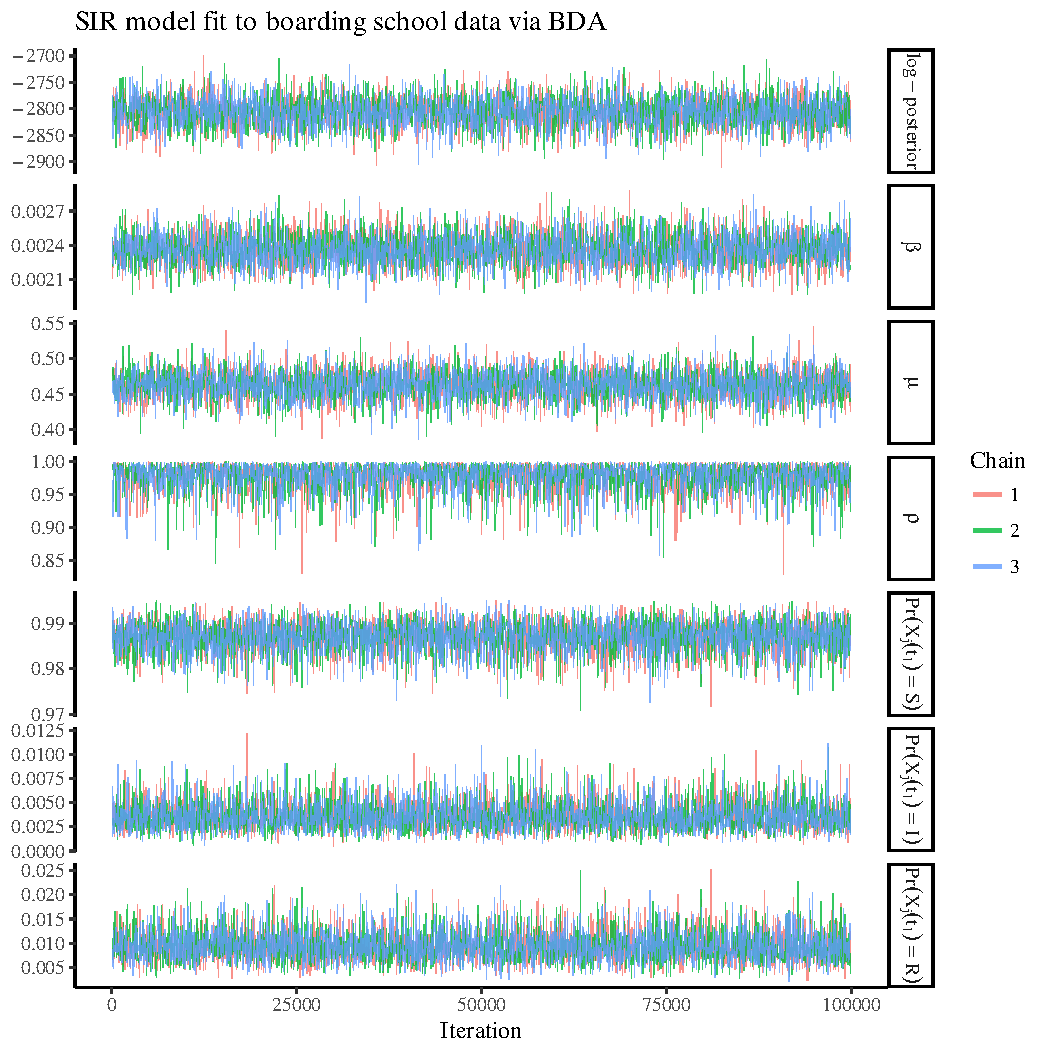
\includegraphics[width=\linewidth]{figures/bbs_sir_bda_traceplots.pdf}
	\caption[Traceplots for SIR model parameters fit to the boarding school data using Bayesian data augmentation.]{Traceplots of the log--posterior and model parameters for the SIR model fit under binomial emissions using BDA following an initial burn--in of 100 iterations. $ \beta $ denotes the per--contact infectivity rate, $ \mu $ is the recovery rate, and $ \rho $ is the binomial sampling probability. Traceplots are thinned to display every 50\textsuperscript{th} iteration.}
	\label{fig:bbs_sir_bda_traceplots}
\end{figure}

\begin{figure}[htbp]
	\centering
	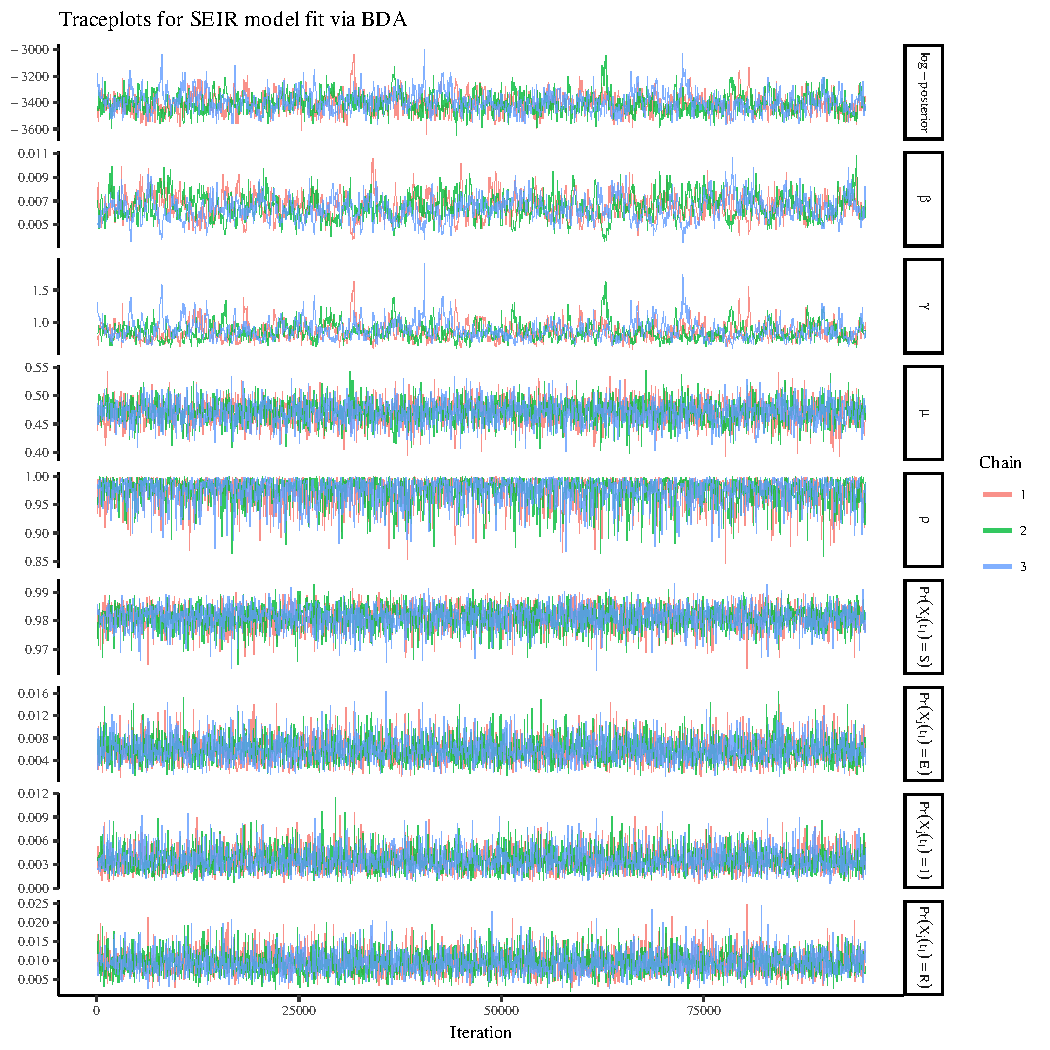
\includegraphics[width=\linewidth]{figures/bbs_seir_bda_traceplots.pdf}
	\caption[Traceplots for SEIR model parameters fit to the boarding school data using Bayesian data augmentation.]{Traceplots of the log--posterior and model parameters for the SEIR model fit under binomial emissions via BDA following an initial burn--in of 5,000 iterations. $ \beta $ denotes the per--contact infectivity rate, $ \mu $ is the recovery rate, $ \gamma $ is the rate at which immunity is lost, and $ \rho $ is the binomial sampling probability. Traceplots are thinned to display every 50\textsuperscript{th} iteration.}
	\label{fig:bbs_seir_bda_traceplots}
\end{figure}

\begin{figure}[htbp]
	\centering
	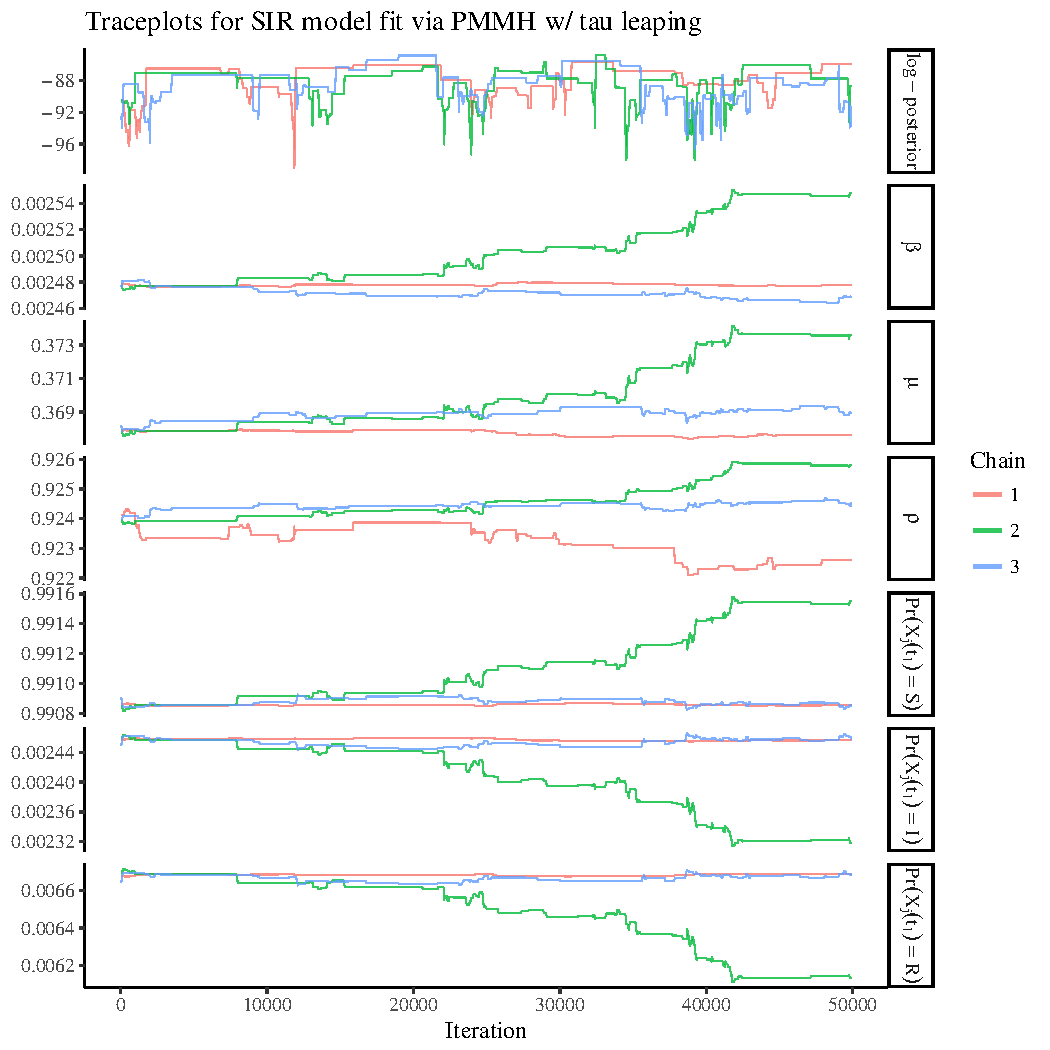
\includegraphics[width=\linewidth]{figures/bbs_sir_pmmh_traceplots.pdf}
	\caption[Traceplots for SIR model parameters fit to the boarding school data using PMMH.]{Traceplots of the log--posterior and model parameters for the SIR model fit under binomial emissions using PMMH with 5,000 particles per chain and a time--step of 2 hours in the approximate $ \tau $--leaping algorithm, following a tuning run of 2,000 iterations to estimate the RWMH covariance matrix and in initial burn--in of 100 iterations. $ \beta $ denotes the per--contact infectivity rate, $ \mu $ is the recovery rate, and $ \rho $ is the binomial sampling probability. Traceplots are thinned to display every 50\textsuperscript{th} iteration.}
	\label{fig:bbs_sir_pmmh_traceplots}
\end{figure}

\begin{figure}[htbp]
	\centering
	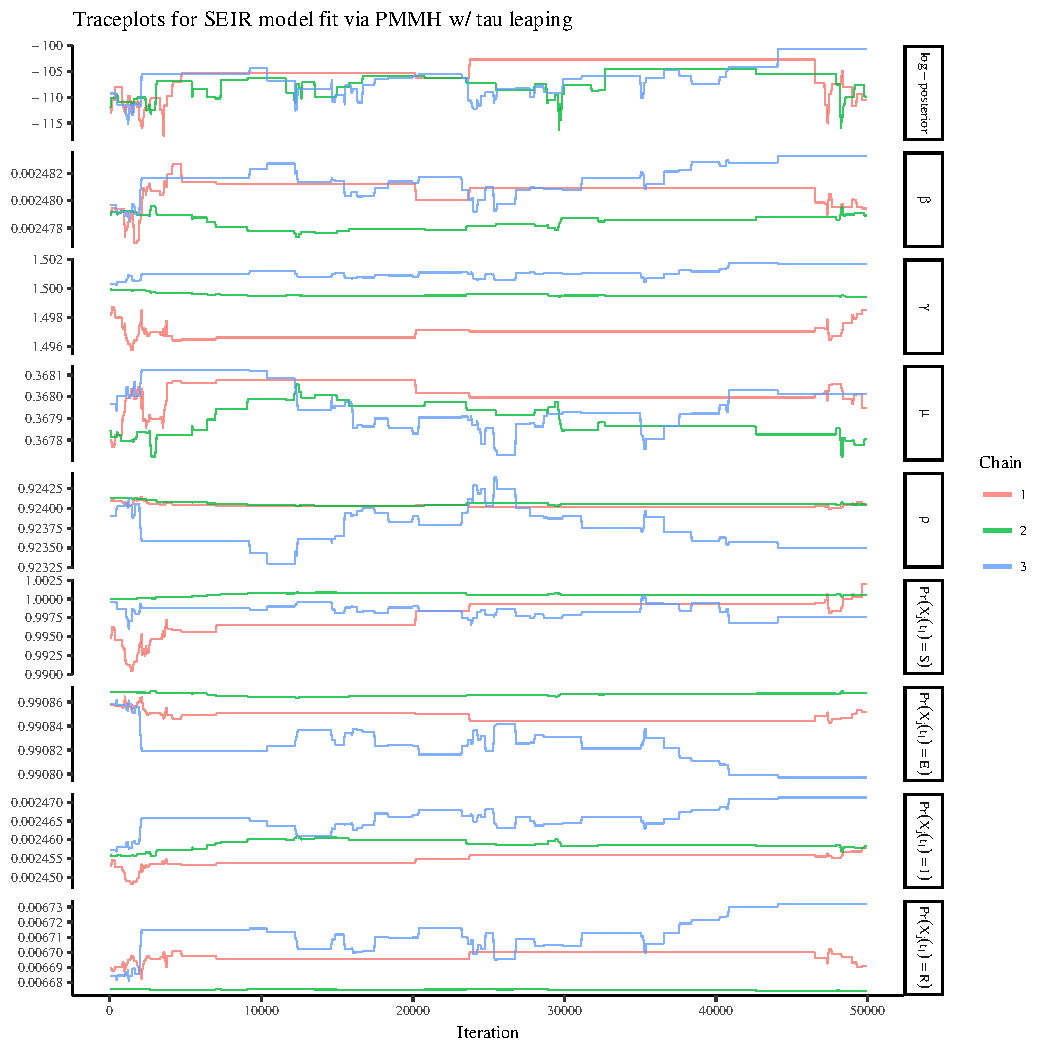
\includegraphics[width=\linewidth]{figures/bbs_seir_pmmh_traceplots.pdf}
	\caption[Traceplots for SEIR model parameters fit to the boarding school data using PMMH.]{Traceplots of the log--posterior and model parameters for the SEIR model fit under binomial emissions using PMMH with 5,000 particles per chain and a time--step of 2 hours in the approximate $ \tau $--leaping algorithm, following a tuning run of 2,000 iterations to estimate the RWMH covariance matrix and in initial burn--in of 100 iterations. $ \beta $ denotes the per--contact infectivity rate, $ \mu $ is the recovery rate, $ \gamma $ is the rate at which immunity is lost, and $ \rho $ is the binomial sampling probability. Traceplots are thinned to display every 50\textsuperscript{th} iteration.}
	\label{fig:bbs_seir_pmmh_traceplots}
\end{figure}

\newpage 

\subsection{Supplementary analysis of the British boarding school example under negative binomial emissions}
\label{sec:bbs_neg_binom}

The PMMH MCMC runs in which SIR and SEIR models were fit to the boarding school data under a binomial emission distribution were plagued by severe particle degeneracy (Figures \ref{fig:bbs_sir_pmmh_traceplots} and \ref{fig:bbs_seir_pmmh_traceplots}). The binomial emission distribution requires that the latent prevalence always be at least as great as the observed prevalence. However, this seemed to be a very stringent criterion with such a high case detection rate. That this criterion was so stringent is suggestive of non--trivial model misspecification. We attempted to confirm this by simulating a dataset that resembled the boarding school data. One possible data generating mechanism that yielded to similar prevalence counts resulted from an outbreak evolving under SEIR dynamics that varied over three epochs (Figure \ref{fig:bbs_dat_sim}). That even a model with this simple set of time--varying dynamics would undoubtedly still be misspecified with respect to the real world circumstances in the boarding school is suggestive of a non--trivial level of model misspecification for both the simple SIR and SEIR models that we attempted to fit. Still, the inability of PMMH to fit simple, easily interpretable, SEMs to this data under binomial emissions is a severe limitation.

\begin{figure}[htbp]
	\centering
	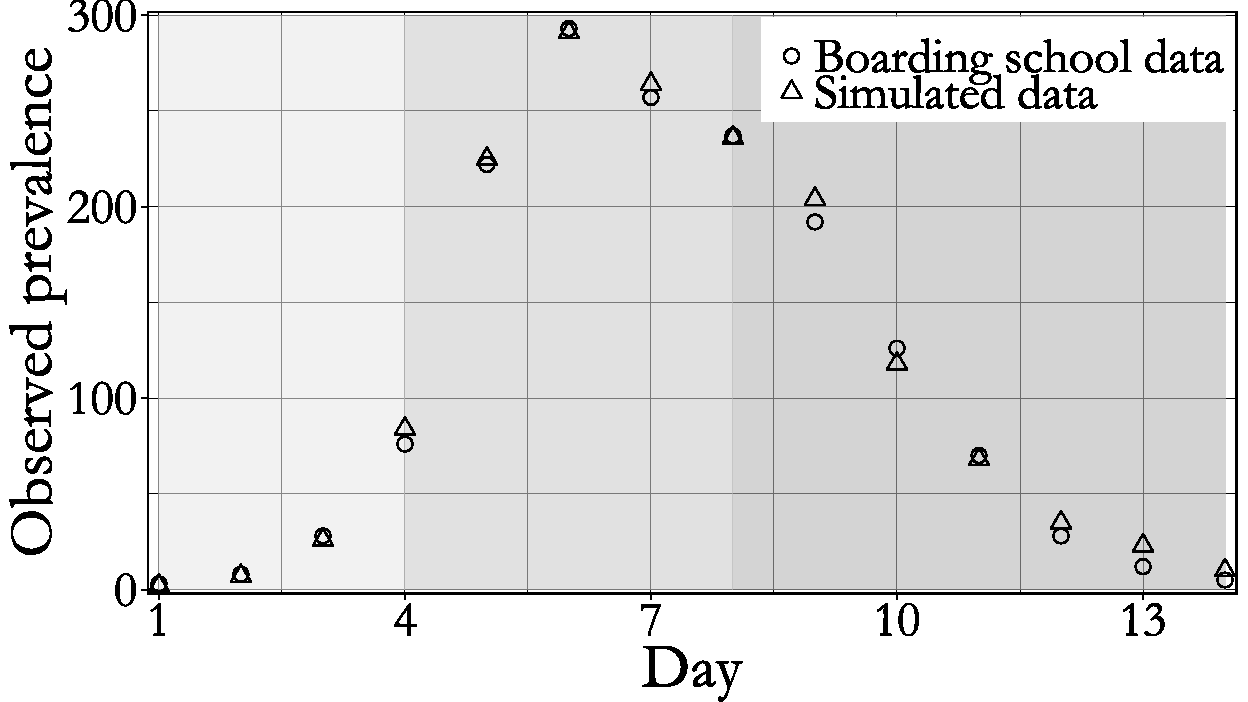
\includegraphics[width=0.6\linewidth]{figures/bbs_dat_sim.pdf}
	\caption[Comparison of boarding school outbreak data and data simulated using an SEIR model with time--varying dynamics.]{British boardings school data and data simulated under SEIR dynamics with time--varying dynamics over three epochs (indicated by different shaded regions). The simulated dataset was generated using the following parameters: in the first epoch (days 1-4), $ \beta = 0.0035,\ \gamma = 1.25,\  \mu = 0.3$. In the second epoch (days 4-8), $ \beta = 0.065,\ \gamma = 0.51,\ \mu = 0.41 $. In the third epoch (days 8-14), $ \beta = 0.06,\ \gamma = 2.5,\ \mu=0.54 $. The data were a binomial sample of the true prevalence with detection probability $ \rho = 0.98 $. There were three exposed individuals and two infected individuals at the beginning of day 1.}
	\label{fig:bbs_dat_sim}
\end{figure}

We fit an alternative set of SIR and SEIR models to the data using BDA and PMMH in which the observed prevalence was modeled as a negative binomial sample of the true prevalence, parameterized by its mean and overdispersion. This is a somewhat unrealistic emission distribution because it allows for the observed prevalence to be greater than the true prevalence. That this tended to occur more often in the later parts of the epidemic when boys were being discharged from the infirmary was particularly odd. However, the negative binomial emission distribution allows us to avoid degeneracy in the collection of PMMH particles by doing away with the constraint that the latent prevalence be no smaller than the observed prevalence. Parameters were assigned the same priors given in Tables \ref{tab:bbs_SIR_prior_binom} and \ref{tab:bbs_SEIR_prior_binom}, and the negative binomial overdispersion parameter, $ \phi $, was assigned a Gamma(1, 0.1) prior parameterized by rate. When fitting the model with BDA, we sampled new values for the rate parameters and initial state probabilities from their univariate full conditional distributions via Gibbs sampling. New values for the negative binomial sampling probability and the overdispersion parameter were sampled using multivariate random walk Metropolis--Hastings on the logit scale for $ \rho $ and on the log scale for $ \phi $. An empirical covariance matrix for the RWMH was estimated from an initial run of 10,000 iterations and scaled until the acceptance rate was between 15\%--50\%. We ran three chains per model for 100,000 iterations each, updating the paths of 100 subjects per MCMC iteration, and discarding the first 10,000 iterations as burn--in. We also ran three chains for 50,000 iterations each using PMMH for each of the models, with 500 particles per chain for the SIR model and 5,000 particles per chain for the SEIR model. Particle paths were simulated approximately using $ \tau $--leaping over a time step of 2 hours. Parameters were updated via multivariate RWMH whose covariance matrix was estimated from an initial tuning run of 2,000 iterations. Rate parameters and the overdispersion parameter were updated on the log scale, the negative binomial sampling probability was updated on the logit scale, and the initial state probabilities were updated on the generalized logit scale. We discarded the first 1,000 of each PMMH chain as burn--in.

\begin{figure}[htbp]
	\centering
	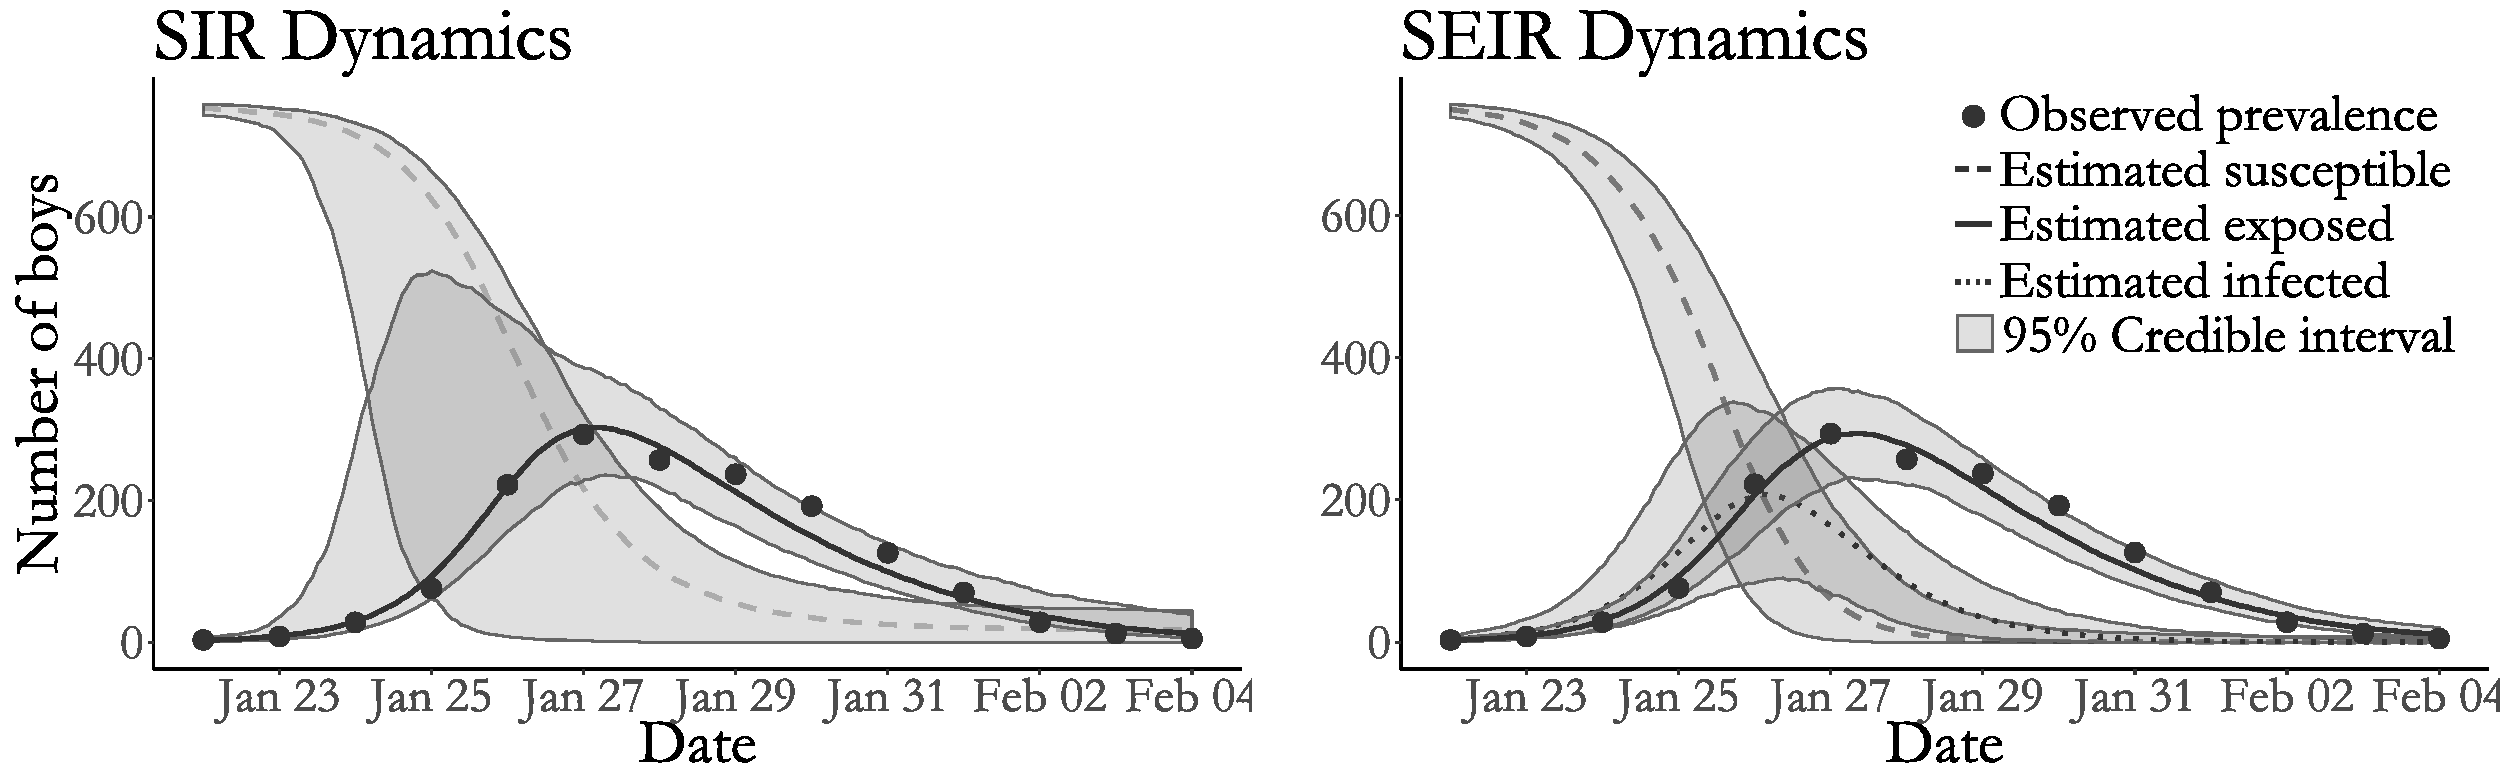
\includegraphics[width=\linewidth]{figures/bbs_latent_post_negbinom.pdf}
	\caption[Latent posterior estimates of prevalence in a boarding school under negative binomial emissions.]{Boarding school data, pointwise posterior median estimates and pointwise 95\% credible intervals under negative binomial emissions (grey shaded areas) for the numbers of infected boys (solid line) and susceptible boys (dashed line). Posterior estimates based on a thinned sample, with every 250$ ^{th} $ configuration retained.}
	\label{fig:bbs_dat_negbinom}
\end{figure}

Although the posterior median estimates under binomial and negative binomial emissions for the SIR and SEIR dynamics and detection rate are generally quite similar, the posterior credible intervals are considerably wider when the data modeled as a negative binomial sample of the true prevalence. This manifests both in the widths of the credible intervals for the latent process (Figure \ref{fig:bbs_dat_negbinom}), and the credible intervals for the model parameters (Figure \ref{fig:bbs_negbinom_credint_comp}). This is not unexpected given that the negative binomial distribution is substantially more flexible than the binomial distribution. In comparing the posterior estimates obtained using BDA and PMMH under negative binomial emissions, we find that the estimates are essentially identical for the SIR model. For the SEIR model, estimates of the dynamics are generally similar, though not to the same degree as those for the SIR model. We notice that the credible intervals for the mean infectious period and the negative binomial detection probability obtained using PMMH are substantially wider than those obtained using BDA. Upon closer inspection of the traceplots of the model parameters, it is clear that the negative binomial overdispersion parameter in the PMMH chains did not converge (Figure \ref{fig:bbs_seir_bda_negbinom_traceplots}).

\begin{figure}[htbp]
	\centering
	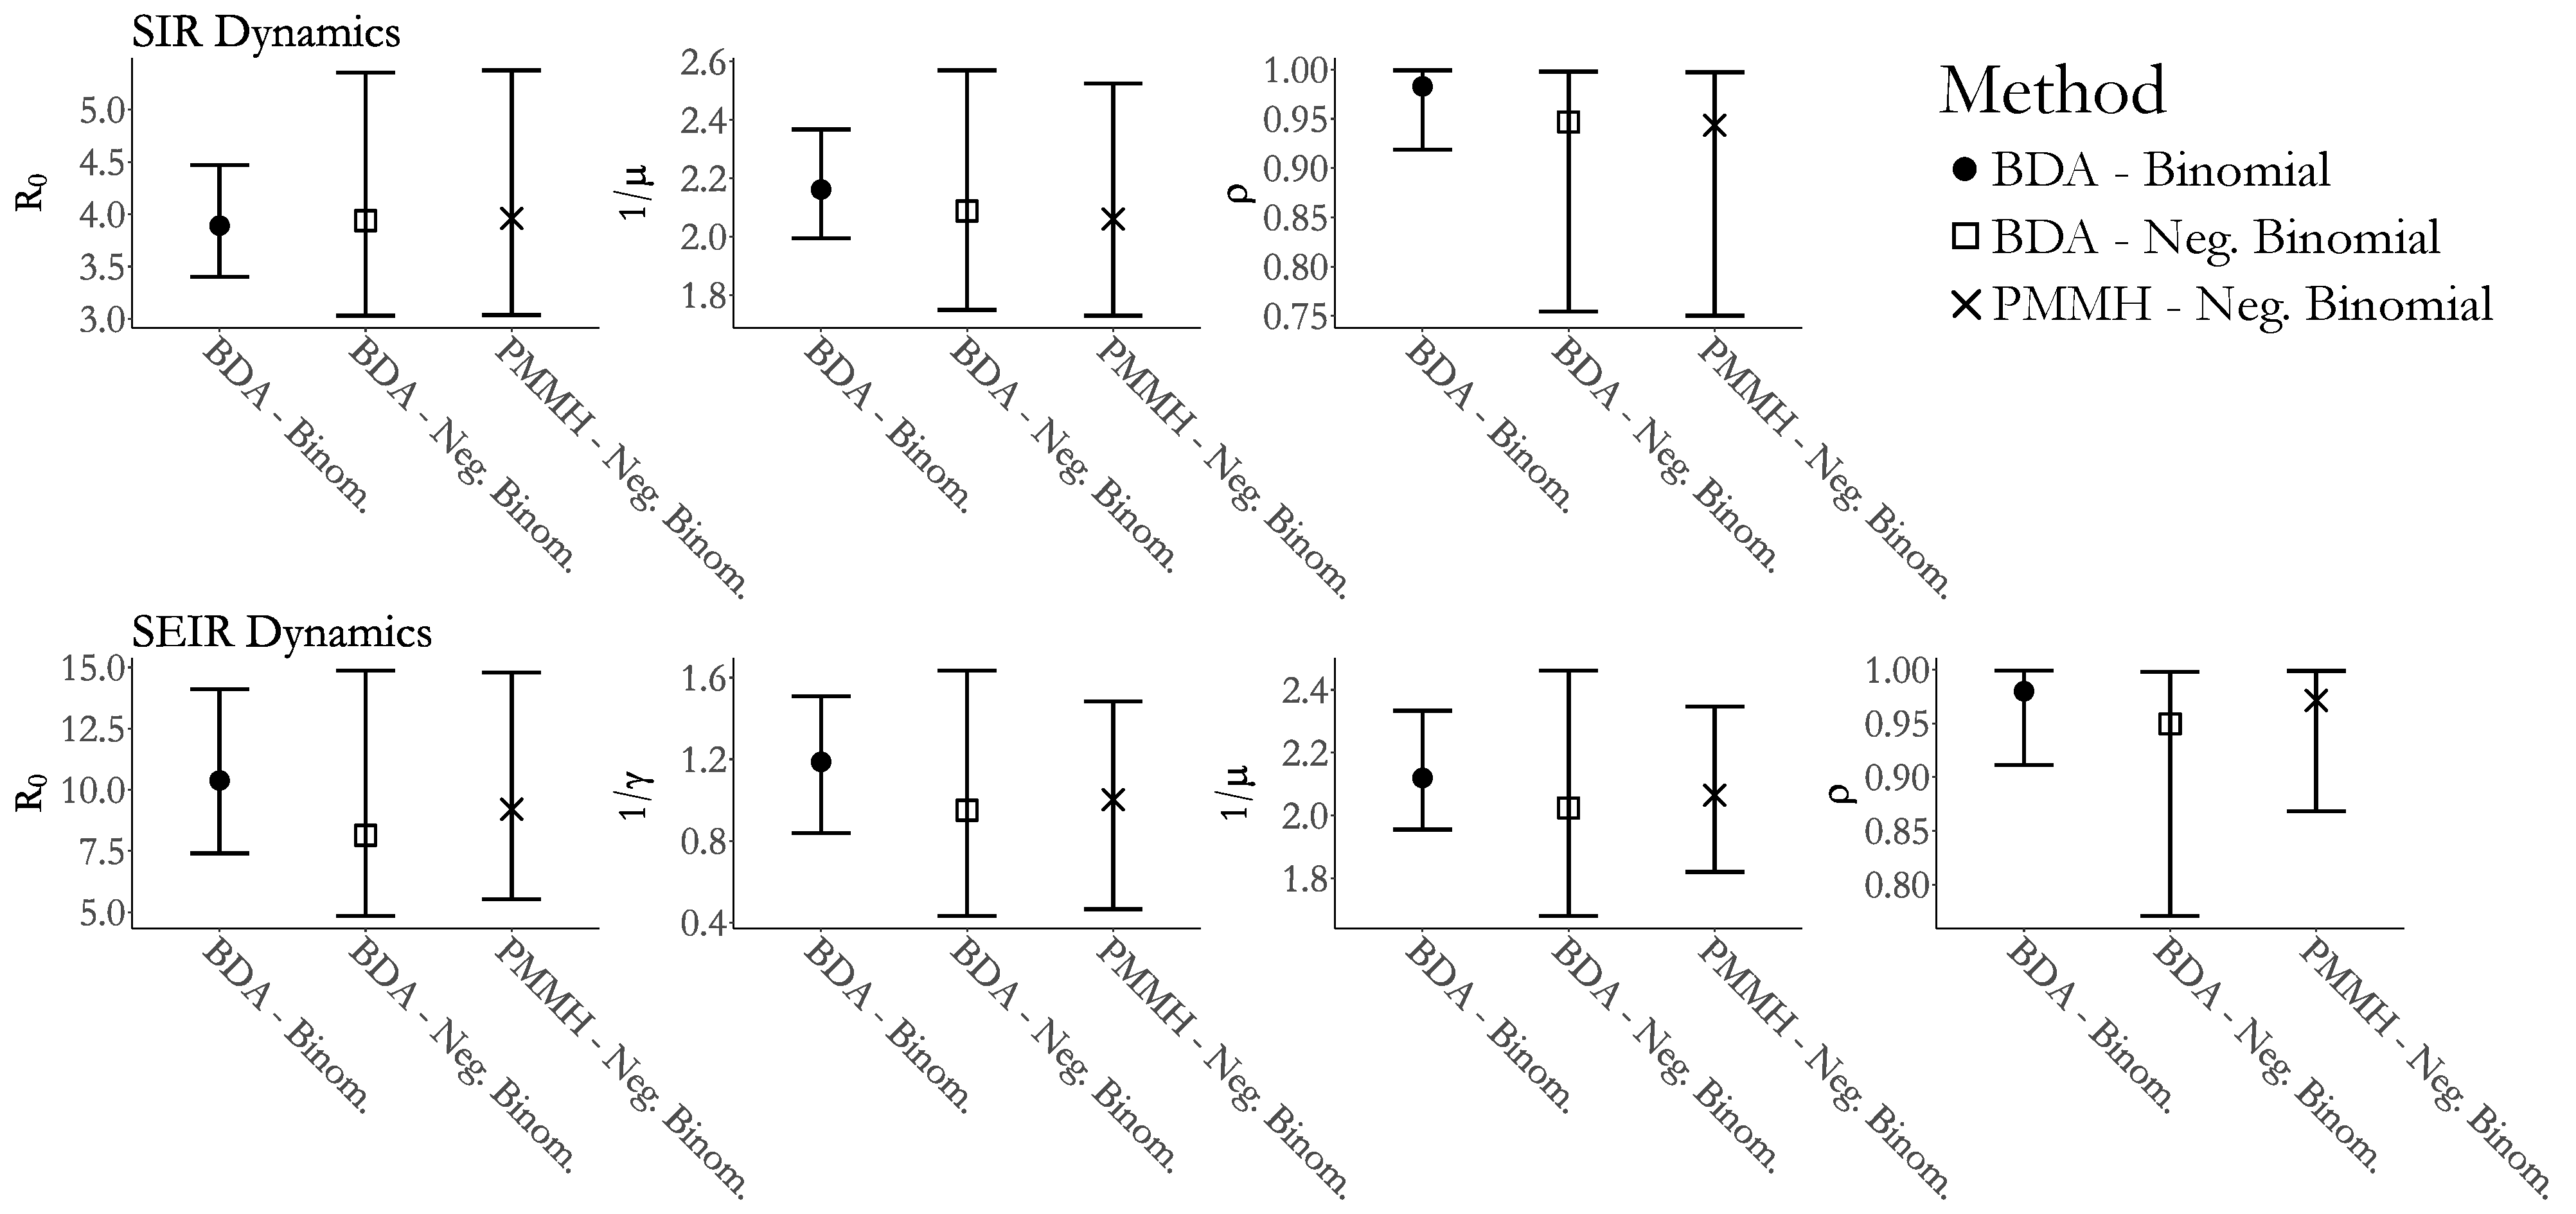
\includegraphics[width=\linewidth]{figures/bbs_negbinom_credint_comp.pdf}
	\caption[Posterior estimates of SIR and SEIR model parameters for models fit under negative binomial emissions.]{Posterior medians and 95\% credible intervals for SIR and SEIR models fit with BDA and PMMH to the British boarding school data under binomial and negative binomial emission distributions.}
	\label{fig:bbs_negbinom_credint_comp}
\end{figure}


\begin{figure}[htbp]
	\centering
	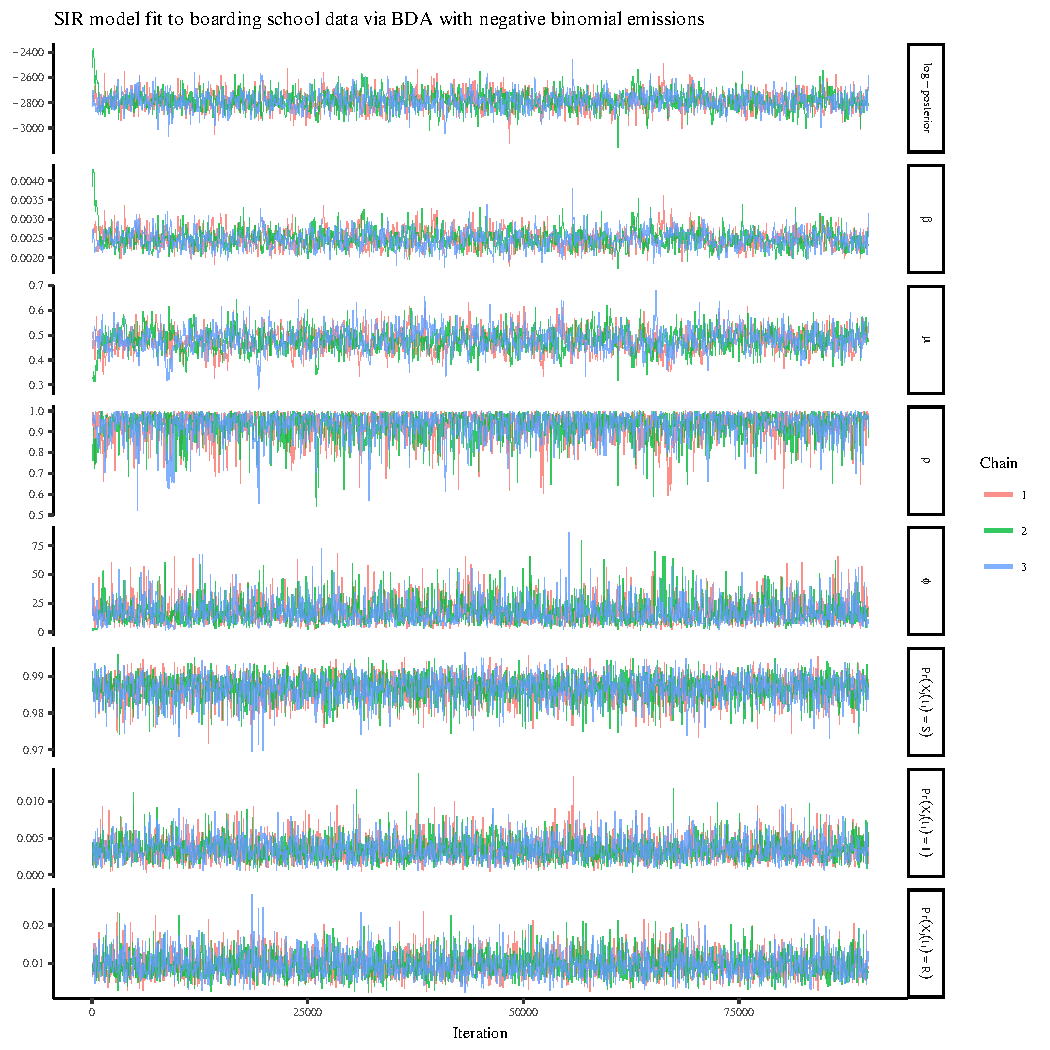
\includegraphics[width=\linewidth]{figures/bbs_sir_bda_negbinom_traceplots.pdf}
	\caption[Traceplots of SIR model parameters fit to boarding school data using Bayesian data augmentation.]{Traceplots of the log--posterior and model parameters for the SIR model fit under negative binomial emissions using BDA following an initial burn--in of 100 iterations. $ \beta $ denotes the per--contact infectivity rate, $ \mu $ is the recovery rate, and $ \rho $ is the binomial sampling probability. Traceplots are thinned to display every 50\textsuperscript{th} iteration.}
	\label{fig:bbs_sir_bda_negbinom_traceplots}
\end{figure}

\begin{figure}[htbp]
	\centering
	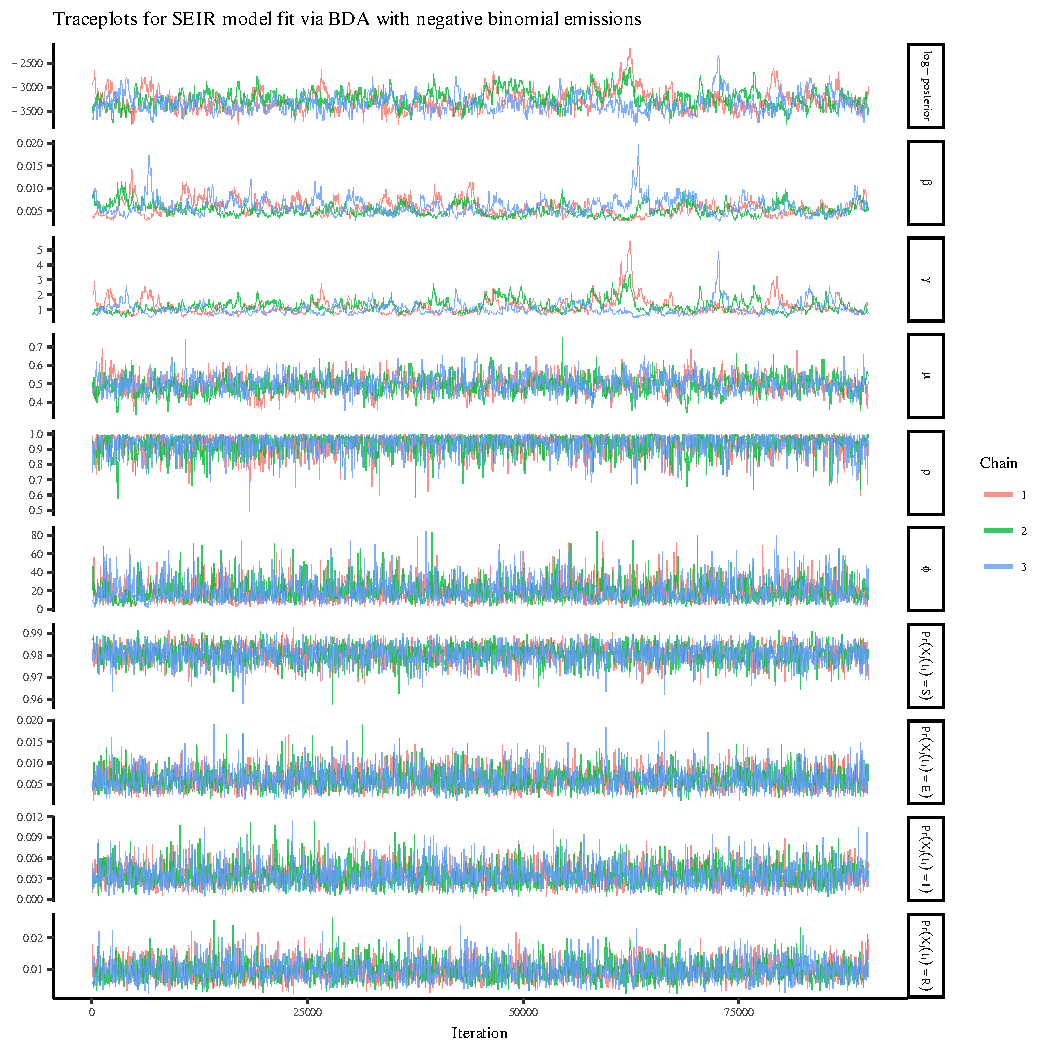
\includegraphics[width=\linewidth]{figures/bbs_seir_bda_negbinom_traceplots.pdf}
	\caption[Traceplots of SEIR model parameters fit to boarding school data using Bayesian data augmentation.]{Traceplots of the log--posterior and model parameters for the SEIR model fit under negative binomial emissions via BDA following an initial burn--in of 5,000 iterations. $ \beta $ denotes the per--contact infectivity rate, $ \mu $ is the recovery rate, $ \gamma $ is the rate at which immunity is lost, and $ \rho $ is the binomial sampling probability. Traceplots are thinned to display every 50\textsuperscript{th} iteration.}
	\label{fig:bbs_seir_bda_negbinom_traceplots}
\end{figure}

\begin{figure}[htbp]
	\centering
	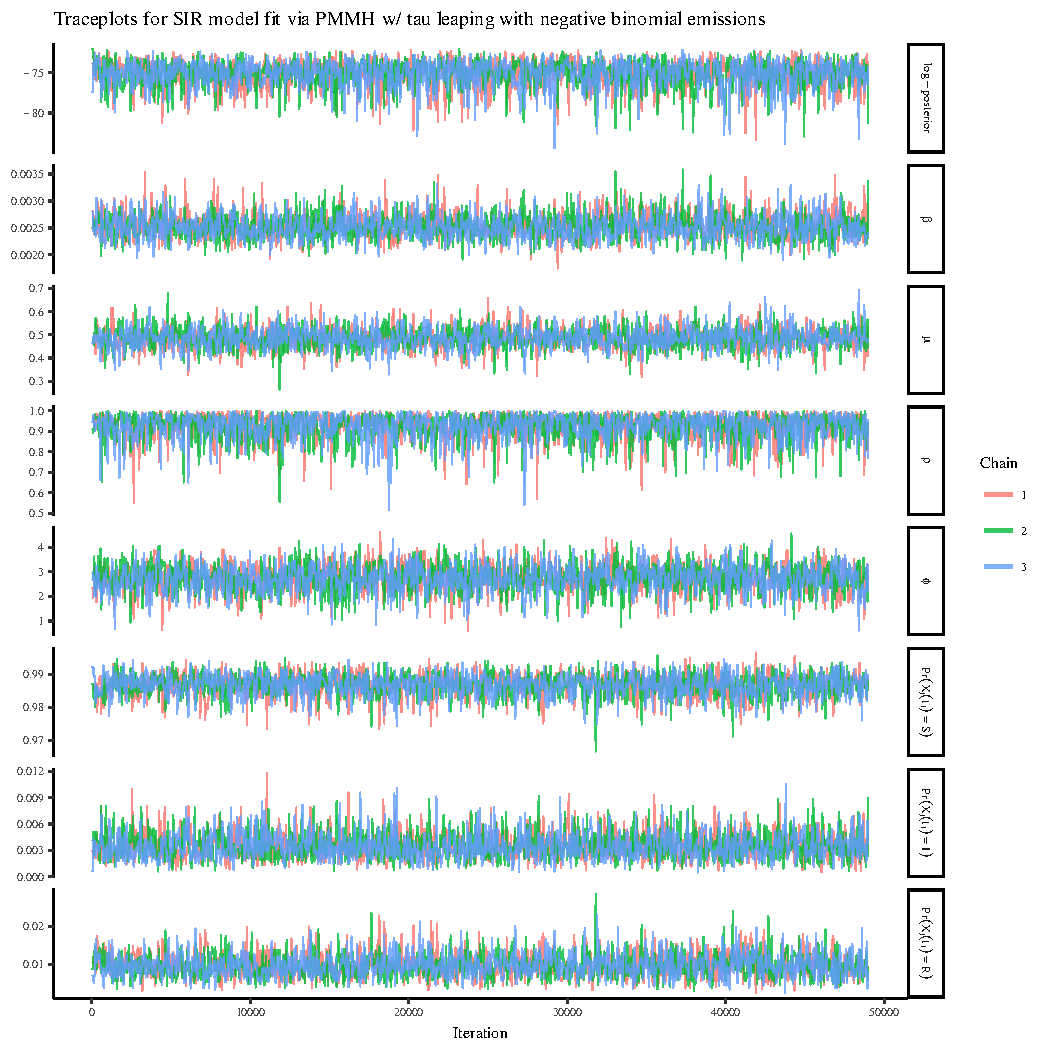
\includegraphics[width=\linewidth]{figures/bbs_sir_pmmh_negbinom_traceplots.pdf}
	\caption[Traceplots of SIR model parameters fit to boarding school data using PMMH.]{Traceplots of the log--posterior and model parameters for the SIR model fit under negative binomial emissions using PMMH with 5,000 particles per chain and a time--step of 2 hours in the approximate $ \tau $--leaping algorithm, following a tuning run of 2,000 iterations to estimate the RWMH covariance matrix and in initial burn--in of 100 iterations. $ \beta $ denotes the per--contact infectivity rate, $ \mu $ is the recovery rate, and $ \rho $ is the binomial sampling probability. Traceplots are thinned to display every 50\textsuperscript{th} iteration.}
	\label{fig:bbs_sir_pmmh_negbinom_traceplots}
\end{figure}

\begin{figure}[htbp]
	\centering
	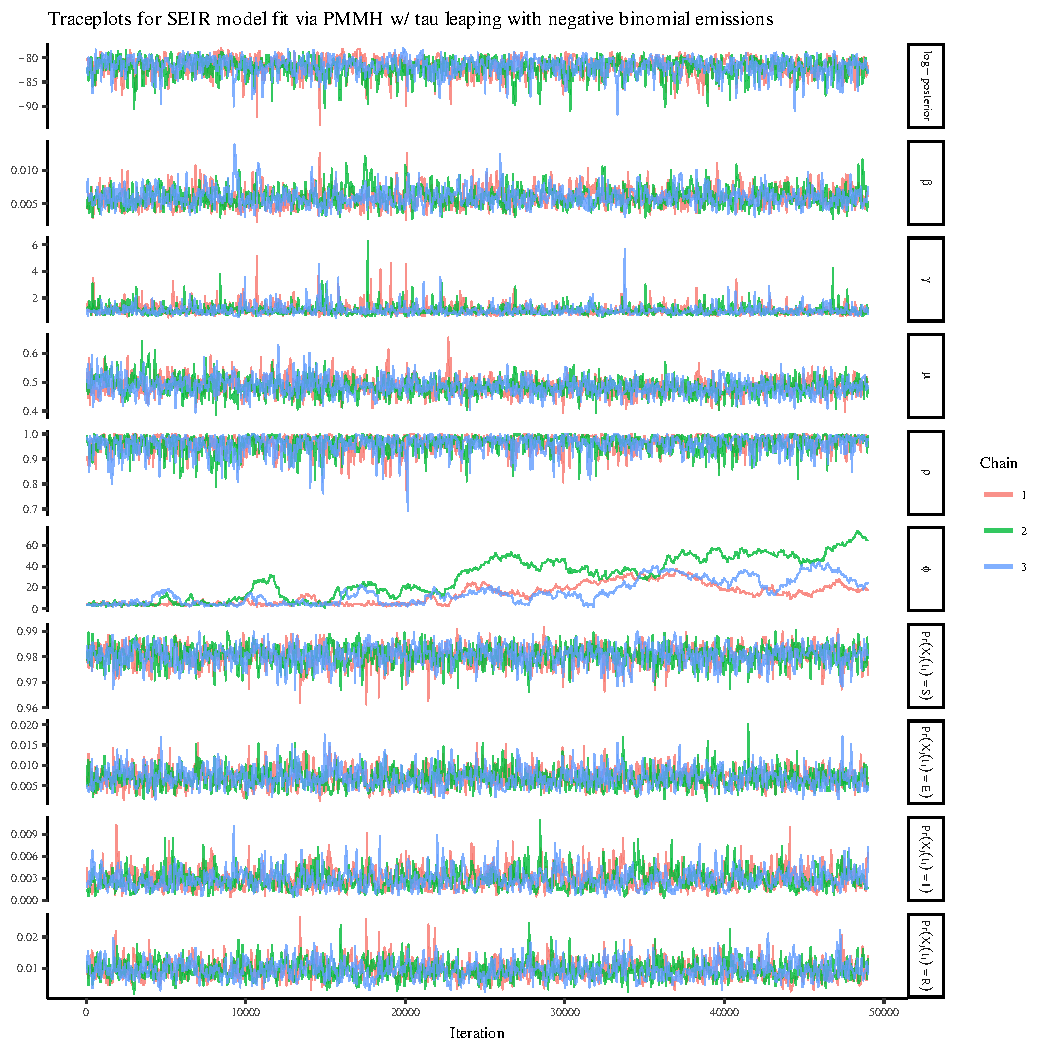
\includegraphics[width=\linewidth]{figures/bbs_seir_pmmh_negbinom_traceplots.pdf}
	\caption[Traceplots of SEIR model parameters fit to boarding school data using PMMH.]{Traceplots of the log--posterior and model parameters for the SEIR model fit under negative binomial emissions using PMMH with 5,000 particles per chain and a time--step of 2 hours in the approximate $ \tau $--leaping algorithm, following a tuning run of 2,000 iterations to estimate the RWMH covariance matrix and in initial burn--in of 100 iterations. $ \beta $ denotes the per--contact infectivity rate, $ \mu $ is the recovery rate, $ \gamma $ is the rate at which immunity is lost, and $ \rho $ is the binomial sampling probability. Traceplots are thinned to display every 50\textsuperscript{th} iteration.}
	\label{fig:bbs_seir_pmmh_negbinom_traceplots}
\end{figure}
